\documentclass[12pt]{report}

\usepackage[utf8]{inputenc}
\usepackage[T1]{fontenc}

\usepackage{mathptmx}
\usepackage{inconsolata}

\usepackage[a4paper, margin=25mm]{geometry}

\usepackage{setspace} \onehalfspace

\usepackage[hidelinks]{hyperref}

\usepackage[estonian]{babel}
\addto\captionsestonian{%
  \renewcommand{\refname}{Viidatud kirjandus}%
  \renewcommand{\appendixname}{Lisad}%
}

\usepackage{todonotes}
\newcommand{\TODO}{\todo[inline]}

\usepackage{amsmath}
\usepackage{amsthm}
\usepackage{amssymb}

\usepackage{booktabs}

% \newcommand*{\YQUANTON}{}
\ifdefined\YQUANTON
  \usepackage{yquant}
\else \fi

\def\yquantjoonis#1{
  \ifdefined\YQUANTON
    {#1}
  \else
    {[joonis]}
  \fi
}

\def\paren#1{\left(#1\right)}
\def\sparen#1{\left[#1\right]}

\def\abs#1{\left|#1\right|}

\def\ket#1{\mathinner{|#1\rangle}}
\def\bra#1{\mathinner{\langle#1|}}

\def\CNOT{\mathop{\mathrm{CNOT}}\nolimits}
\def\SWAP{\mathop{\mathrm{SWAP}}\nolimits}
\def\cnot{\mathop{\mathrm{CNOT}}\nolimits}
\def\swap{\mathop{\mathrm{SWAP}}\nolimits}

\def\QFT{\mathop{\mathrm{QFT}}\nolimits}


\newcommand{\comment}[1]{}

\usepackage[style=numeric]{biblatex}
\addbibresource{srcs.bib}

\begin{document}

\tableofcontents


\chapter{Sissejuhatus}

Kvantarvutuste valdkonna üks peamine arengumotivatsioon on alati olnud soov simuleerida keerulisi kvantsüteeme.
Juba 1980ndatel, kui kvantarvutuste valdkond oli alles tekkimas, käisid Juri Manin ja Richard Feynman teineteiest eraldi välja idee, et kvantsüsteemide simulateerimise ülesannete lahendamiseks võiksid hästi sobida just kvantarvutid~\cite{manin, feynman}.

Simulatsiooniülesande saab analüütiliselt lahendada vaid lihtsaimate kvantsüsteemide jaoks, mille tuntuimad näited on harmooniline ostsillaator ja vesiniku aatom.
Keerukamate süsteemide klassikaliseks simuleerimiseks kasutatakse numbriliseid meetodeid~\cite{whitfield+etal2011, szabo+ostlund}.

Kvantsüsteemi simuleerimisülesande klassikaline lahendamine on aga möödapääsmatult ebaefektiivne: Schrödingeri võrrandi klassikalise lahendamise ressursikulu sõltub süsteemi suurusest eksponentsiaalselt~\cite{whitfield+etal2011, mcardle+etal, cao+etal, kassal+etal}.
Klassikaliselt ei pruugi suuremaid ülesandeid olla kunagi võimalik lahendada, ammugi täpselt.

Samas on teada mitu tähtsat kvantalgoritmi, mille teoreetiline efektiivsus ületab klassikalise analoogi oma.
Arvatakse, et nende algoritmidega saab tulevikus lahendada ülesandeid, mille klassikalist lahendamist peetakse jäädavalt liiga kulukaks.
Need algoritmid on võimalikud tänu kvantarvutuse ainulaadsetele vahenditele.

Kvantsimulatsioon on kvantsüsteemide simuleerimine kvantarvutuslikult.
Et kvantarvuti on ju ka ise kvantsüsteem, siis on sellega võimalik soodsalt simuleerida uuritava kvantsüsteemi dünaamikat.
Seda arvasid juba Manin ja Feynman~\cite{manin, feynman}.
Eelis klassikalise simuleerimise ees on eksponentsiaalne~\cite{whitfield+etal2011, mcardle+etal, cao+etal}.

Siiani on kvantarvututitega õnnestunud lahendada vaid mõni üksik selline probleem, mille lahendamine on klassikaliste arvutitega on praktiliselt võimatu.
Nimelt takistab kvantarvutite kasutamist nende ebatäiuslik riistvara: arvutuste käigus tekib müra~\cite{whitfield+etal2022}.

Siiski on kvantalgoritm mõtekas uurida tuleviku tarvis, sest kvantarvutite riistvara areneb pidevalt.
Pretsedentdiks on klassikaliste arvutite kiire areng.
Lähemas tulevikus võib õnnesuda kasutada hübriidalgoritme, mis põhinevad kvantarvutite ja klassikaliste arvutite koostööl~\cite{omalley+etal}.

Käesoleva töö eesmärgiks on demonstreerida klassikalisest efektiivsemat kvantarvutusliku meetodid molekulaarse hamiltoniaani simuleerimiseks.
See meetod põhineb faasi hindamise algoritmil.
Süsteemiks on vesiniku molekul \(\rm H_2\), ülesandeks on põhienergia leidmin kui näide elektronstruktuuri ülesandest.

Lahendamine algab klassikaliste eelarvutustega, mida tutvustab peatükk~\ref{chap:qchem}.
Eelarvutuste tulemuseks on Focki ruumi hamiltoniaan teise kvantiseerimise kujul.

Peatkükk~\ref{chap:qcomp} käsitleb ülesande kvantarvutusliku lahendamist.
Sammud lahendamiseks on järgmsised~\cite{whitfield+etal2011}.

\begin{enumerate}
    \item Focki ruumi molekulaarne hamiltoniaan tuleb esitada kvantbittide ruumis.
    Seda käsitleb alapeatükk~\ref{sec:jw}.
    \item Kvantbittide ruumis esitatud molekulaarse hamiltoniaani põhjal tuleb koostada ajalise arengu operaator ja realiseerida see kvantväravana.
    Seda käsitleb alepeatükk~\ref{sec:qcirc}.
    \item Ajalise arengu operaatori omaväärtused saab leida kasutades faasi hindamise algoritmi.
    Seda käsitleb alepeatükk~\ref{sec:pea}.
\end{enumerate}
Selguse huvides on sammud tekstis esitatud vastupidises järjekorras.

Selles töös on arvutuste läbiviimiseks kasutatud simulaatorit.
Kasutatud vahendeid käsitleb peatükk~\ref{chap:methods}.
Peatükk~\ref{chap:results} tutvustab tulemusi.

\chapter{Elektronstruktuuri ülesanne}

\section{Molekulaarse süsteemi hamiltoniaani üldkuju}

Molekuli keemilised omadused määrab elektronstruktuur.
Tuumade mõju pole üldjuhul oluline.
Siin töös pakubki huvi vaid elektronstruktuur, mida kirjeldab elektronide hamiltoniaan.

Et elektronide ja tuumade dünaamika pole sõltumatu, siis ei saa elektronide hamiltoniaani aprioorselt kirja panna.

Molekuli kui terviku hamiltoniaan on
\begin{align}\label{eq:molham}
    H_\text{mol} = \underbrace{\sum_{i = 1}^N \frac{1}{2} \nabla_i^2}_\text{(a)}
    \underbrace{- \sum_{A = 1}^M \frac{1}{2 M_A} \nabla_A^2}_\text{(b)}
    \underbrace{- \sum_{i = 1}^N \sum_{A = 1}^M \frac{Z_A}{r_{iA}}}_\text{(c)}
    \underbrace{+ \sum_{i = 1}^N \sum_{j > i}^N \frac{1}{r_{ij}}}_\text{(d)}
    \underbrace{+ \sum_{A = 1}^M \sum_{B > A}^M \frac{Z_A Z_B}{r_{AB}}}_\text{(e)} \rlap{,}
\end{align}
kus \(M_A\) on tuuma \(A\) ja elektroni massi suhe, \(Z_A\) on tuuma \(A\) aatomnumber, \(r_{ij}\) on elektronide \(i\) ja \(j\) vahekaugus ning \(R_{AB}\) on tuumade \(A\) ja \(B\) vahekaugus.
Valemis esinevad järgmised liimed: (a) on elektronide kineetilise energia liige, (b) tuumade kineetilise energia liige, (c) elektronide ja tuumade tõmbumise liige, (d) elektrinode omavahelise tõukumise operaator ja (e) tuumade omavahelise tõukumise liige.
See valem kirjeldab nii tuumasid kui ka elektrone~\cite{szabo+ostlund}.

Elektronide hamiltoniaani saamiseks tuleb valemist~\eqref{eq:molham} eraldada elektronide osa.

\section{Born-Oppenheimeri lähendus}\label{sec:bo}

Valemist~\eqref{eq:molham} elektronide osa eraldamiseks tehakse kvantkeemias keskne Born-Oppeheimeri lähendus, mille põhimõtte on järgmine.

Et tuumad on palju raskemad kui elektronid, siis liiguvad tuumad elektronidega võrreldes palju aeglasemalt.
Born-Oppenheimeri lähenduses on tuumad üldse paigal: elektronid liiguvad tuumade tekitatud statsionaarses väljas~\cite{szabo+ostlund}.

Selles lähenduses kaob valemist~\eqref{eq:molham} tuumade kineetilise energia liige~(b)~\cite{szabo+ostlund}.

Tuumade omavahelise tõmbumise liige~(e) on aga konstante.
Et konstandi võrra erinevatel operaatoritel on samad omafunktsioonid, võib liikme~(e) üldse arvestamata jätta~\cite{szabo+ostlund}.

Tulemuseks on vaid elektronkatet kirjeldav hamiltoniaan
\begin{align}\label{eq:elham}
    H_\text{elek} = \underbrace{\sum_{i = 1}^N \frac{1}{2} \nabla_i^2}_\text{(a)}
    \underbrace{- \sum_{i = 1}^N \sum_{A = 1}^M \frac{Z_A}{r_{iA}}}_\text{(c)}
    \underbrace{+ \sum_{i = 1}^N \sum_{j > i}^N \frac{1}{r_{ij}}}_\text{(d)} \rlap{,}
\end{align}
mida kutsutaksegi elektronide hamiltoniaaniks~\cite{szabo+ostlund}.

Hamiltoniaan~\eqref{eq:elham} erineb küll hamiltoniaanist~\eqref{eq:molham} omaväärtuste poolest, kuid kehtib
\begin{align}
    E_\text{mol} = E_\text{elek} + E_\text{tuum} \rlap{,}
\end{align}
kus \(E_\text{mol}\) on vana ja \(E_\text{elek}\) uue hamiltoniaani omaväärtus.
\(E_\text{mol}\) on molekuli kui terviku energia.
\(E_\text{elek}\) on elektronkatte energia.
\(E_\text{tuum}\) on tuumade energia, mille võrra~\eqref{eq:elham} ja \eqref{eq:molham} omaväärtused erinevad.
Elektronstruktuuri ülesandes pakubki aga huvi vaid \(E_\text{elek}\)~\cite{szabo+ostlund}.

Edaspidi tähsitame \(H = H_\text{elek}\) ja \(E = E_\text{elek}\).

Valemit~\eqref{eq:elham} on vaja edasi lihtsutada, sest hetkel on tegemist mitme keha probleemiga.

\section{Hartree korrutis ja Slateri determinant}\label{sec:hpsd}

See alapeatükk keskendub elektronkatte lainefunktsioonile, milleks on kaks põhjust.
Esiteks on vaja lainefunktsiooni täpsustada valemi~\eqref{eq:elham} edasiseks lihtsustamiseks.
Teiseks on hiljem vaja teada põhioleku lainefunktsiooni kuju, et leida põhioleku energia.

Lainefunktsiooni \(\Psi\) jaoks on kaks tingimust.
Ühest küljest peab see rahuldama Scrödingeri võrrandit
\begin{align}
    H_\text{elek} \Psi = E_\text{elek} \Psi \rlap{.}
\end{align}
Teisalt peab see rahuldama antisümmetria printsiipi
\begin{align}
    \Psi(\vec{x_1}, \ldots, \vec{x_i}, \ldots, \vec{x_j}, \ldots, \vec{x_N})
    = -\Psi(\vec{x_1}, \ldots, \vec{x_j}, \ldots, \vec{x_i}, \ldots, \vec{x_N}) \rlap{,}
\end{align}
kus \(\vec{x_1}\) kuni \(\vec{x_N}\) on osakeste \(1\) kuni \(N\) üldised koordinaadid, mis sisaldavad informatsiooni nii osakeste asukohtade kui ka spinnide kohta.
Antiümmeetria printsiib on Pauli keelu printsiibi üldisem sõnastus~\cite{szabo+ostlund}.

Sobiva lainefunktsiooni saab molekulaarobitaalide teooriast.

Selles teoorias nimetatakse spinnorbitaaliks funktsiooni
\begin{align}\label{eq:spinorb}
    \chi_j(\vec{x_i}) = \begin{cases}
        \alpha(\omega_i) \phi_j(\vec{r_i})\text{,} & \text{kui \(i\) ei jagu \(2\)-ga} \\
        \beta(\omega_i) \phi_{j-1}(\vec{r_i})\text{,} & \text{kui \(i\) jagub \(2\)-ga} \\
    \end{cases}
\end{align}
Spinnorbitaal on ühe elektroniga moleklulaarse süsteemi lainefunktsiooniks.
Valemis~\eqref{eq:spinorb} on \(x_i\) elektroni \(i\) üldine koordinaat, mis koosneb kahest osast: \(\omega_i\) kirjeldab selle elektroni spinni, \(\vec{r_i}\) ruumilist paiknemist.
\(\alpha(\omega_i)\) vastab spinn-alla olukorrale ja \(\beta(\omega_i)\) spinn-üles olukorrale.
\(x_j(x_i)\) on ruumiline orbitaal ehk elektroni lainefunktsioon, mis ei arvesta spinni.
Iga ruumilise orbitaali kohta on võimalik kaks spinnorbitaali~\cite{szabo+ostlund}.

Spinnorbitaalide korrutist
\begin{align}\label{eq:hp}
    \Psi^\text{HP}(\vec{x_1}, x_2, \ldots, \vec{x_N})
    = \chi_i(\vec{x_1}) \chi_j(\vec{x_2}) \cdots \chi_i(\vec{x_N})
\end{align}
nimetatakse Hartree korrutiseks.
Kui antisümmeetria printsiipi poleks vaja arvestada, siis oleks Hartree korrutis teineteisega mitteinterakteeruvate elektronidega süsteemi lainefunktsiooniks.
Näitame seda.

Sellisel lihtsustatud juhul oleks elektronid sõltumatud: süsteemi hamiltoniaani saaks kirja panna kujul
\begin{align}
    H = \sum_i^N h(i) \rlap{,}
\end{align}
kus \(h(i)\) on iga üksiku elektroni hamiltoniaan.
Et kehtib
\begin{align}
    E = \sum_i^N \epsilon_i \rlap{,}
    \qquad \text{kus} \qquad
    H \Psi^\text{HP} = E \Psi^\text{HP}
    \quad \text{ja} \quad
    h(i) \chi_j(\vec{x_i}) = \epsilon_j \chi_j(\vec{x_i})
\end{align}
siis sellise süsteemi koguenergia oleks üksikute elektronide energiate summa, mis näitabki Hartree korrutise sobivust lainefunktsiooniks mitme elektroniga süsteemi lihtsustatud juhul.

Kuigi me seda siin ei näita, siis arvestab antisümmeetria printsiipi ja elektronide vastasmõju Hartree korrutise edasiarendus
\begin{align}\label{eq:slater}
    \Psi(\vec{x_1}, \vec{x_2}, \ldots, \vec{x_n})
    = \frac{1}{\sqrt{N!}} \begin{vmatrix}
        \chi_i(\vec{x_1}) & \chi_j(\vec{x_2}) & \cdots & \chi_k(\vec{x_2}) \\
        \chi_i(\vec{x_2}) & \chi_j(\vec{x_2}) & \cdots & \chi_k(\vec{x_2}) \\
        \vdots & \vdots & & \vdots \\
        \chi_i(\vec{x_N}) & \chi_j(\vec{x_N}) & \cdots & \chi_k(\vec{x_N}) \\
    \end{vmatrix} \rlap{,}
\end{align}
mida kutsutakse Slateri determinandiks.
Pikemalt käsitleb Slateri determinandi omadusi~\cite{szabo+ostlund}.
Oluline on, et Slateri determinant sobib elektronide lainefunktsiooniks.

Slateri determinandi~\eqref{eq:slater} lühitähistus on \(\ket{\chi_i\chi_j\cdots\chi_k}\), mis tähendab, et elektron \(1\) asub spinnorbitaalil \(\chi_i\), elektron \(2\) spinnorbitaalil \(\chi_j\) jne.

\section{Hartree-Focki lähendus}\label{sec:hf}

Alapeatükis~\ref{sec:bo} selgus, et Born-Oppeheimeri lähenduse tulemuseks on mitme keha probleem, mille lahendamine on teadagi keeruline.

Ülesanne muutub ühe keha probleemiks Hartree-Focki lähenduses, kus teise elektronide mõju igale elektronile võetakse arvesse statsionaarse väljana.
See lähendus on kvantkeemias laialt kasutuses ja annab enamasti piisavalt täpse tulemuse~\cite{szabo+ostlund}.

Varasemast teame, et mitme elektroniga süsteemi põhioleku lainefunktsioon on kujul
\begin{align}
    \ket{\Psi_0} = \ket{\chi_1 \chi_2 \cdots \chi_N} \rlap{,}
\end{align}
kus \(N\) on elektronide arv.

Variatsiooni printsiibist tulenevalt on põhioleku lainefunktsioon selline, mille energia
\begin{align}
    E_0 = \bra{\Psi_0} H \ket{\Psi_0} \rlap{.}
\end{align}
on minimaalne.
Energia väärtus sõltub spinnorbitaalide \(\chi_1\), \(\chi_2\), \(\ldots\), \(\chi_N\) valikust~\cite{szabo+ostlund}.

Energia minimeerimine viib valemini
\begin{align}\label{eq:hf}
    f(i) \chi(\vec{x_i}) = \epsilon \chi(\vec{x_i}) \rlap{,}
\end{align}
mida kutsutakse Hartree-Focki võrrandiks~\cite{szabo+ostlund}.

Valmis~\eqref{eq:hf} on
\begin{align}
    f(i) = -\frac{1}{2} \nabla_i^2 - \sum_{A = 1}^M \frac{Z_A}{r_{iA}} + v^\text{HF}(i)
\end{align}
Focki operaator.
Viimases valemis on \(v^\text{HF}(i)\) elektroni \(i\) kogetud keskmine potentsiaal, mis on tingitud teiste elektronide mõjust~\cite{szabo+ostlund}.

Hartree-Focki võrrandi lahendamisprotseduuri me siin ei käsitle, vt~\cite{szabo+ostlund}.

Lahendamise tulemuseks on Hartree-Focki spinnorbitaalide komplekt \(\{\chi_k\}\), millele vastab energiate komplekt \(\{\epsilon_k\}\), kusjuures \(k > N\)~\cite{szabo+ostlund}.

Põhioleku lainefunktsioon on
\begin{align}
    \ket{\Psi_0} = \ket{\chi_a \chi_b \cdots \chi_c} \rlap{,}
\end{align}
kus \(\chi_a\), \(\chi_b\), \(\ldots\), \(\chi_c\) on \(N\) madalaima energiaga spinnorbitaali.
Orbitaale \(\chi_a\), \(\chi_b\), \(\ldots\), \(\chi_c\) nimetakse täidetud orbitaalideks, ülejäänud on virtuaalised orbitaalid.

Spinnorbitaalide kuju sõltub baasifunktsioonide komplekist, mida nimetatakse keemiliseks baasiks.
Sama ülesande lahendamsieks võib kasutada suuremat või väiksemat keemilist baasi.
Väiksemad keemilised baasid on küll ebatäpsemad, kuid need võimaldavad arvutusressurside kokkuhoidu.
Tuntuim keemiline baason STO-3G, mida kutsutakse ka minimaalseks baasiks.

\section{Teine kvantiseerimine}\label{sec:secquant}

Enne Focki ruumist kvantbittide ruumi suundumist, mis on vajalik ülesande kvantarvutuslikuks lahendamiseks, on kasulik esitada hamiltoniaan ja lainefunktsioon teise kvantseerimise kujul.
Teise kvantseerimise kuju võtab arvesse sümmeetria omadusi ja sedasi on võimalik probleemi lihtsustada~\cite{kassal+etal, yung+etal}.

Teise kvantiseerimise formalism ehitatakse üles kahele operaatorile.

Tekkeopraator \(a_i^\dagger\) tekitab süsteemi juurde elektroni spnnorbitaalile \(\chi_i\):
\begin{align}
    a_i^\dagger \ket{\chi_k \cdots \chi_l} = \ket{\chi_i \chi_k \cdots \chi_l} \rlap{.}
\end{align}

Kaooperaatoer \(a_i\) eemaldab süsteemist elektroni spinnorbitaalilt \(\chi_i\):
\begin{align}
    a_i \ket{\chi_i \chi_k \cdots \chi_l} = \ket{\chi_k \cdots \chi_l}\rlap{.}
\end{align}

Tekke- ja kaoperaatori algebralised omadused on kooskõlas determinantide omadustega, mis saavtatakse kommutatsioonireeglitega
\begin{align}
    \sparen{\alpha_i^\dagger, \alpha_j^\dagger} = 0 \rlap{,}
    \qquad \sparen{\alpha_i, \alpha_j} = 0 \rlap{,}
    \qquad \sparen{\alpha_i, \alpha_j^\dagger} = \delta_{ij} \rlap{.}
\end{align}

Teise kvantseerimise kujul antud hamiltoniaani ja lainefunktsiooni viib kvantbittide ruumi Jordan-Wigneri teisendus, mida käsitletakse alapeatükis~\ref{sec:jw}.

\section{Energia leidmine}

Edasine ülesanne on järgmine.

Olgu meil antud molekulaarse süsteemi elektronide hamiltoniaan \(H\).
Ülesandeks on leida olekule pòhiolekule \(\ket{\Psi_0}\) vastav energia \(E\).
Selleks tuleb lahendada omaväärtusvõrrand
\begin{align}
    H \ket{\Psi_0} = E \ket{\Psi_0} \rlap{,}
\end{align}
mis on klassikaliset kulukas ülesanne.
Tegemist on elektronstruktuuri ülesande ühe variandiga.

Järgmise peatatükk tutvustab kvantarvutusliku meetodit selle ülesande lahendamiseks, mis on klassikalisest efektiivsem.
Meetod töötab peale põhioleku ka teiste olekute jaoks.

\chapter{Kvantarvutuslik lahendamine}\label{chap:qcomp}

See peatükk tutvustab kvantahelamudeli põhitõdesid ja paneb paika tähistuse,
mis leiab kasutust hilisemates peatükkides. Samuti on siin ära toodud mõned
kvantarvutite eelised klassikaliste arvutite ees, põhjendatud, miks
kvantarvutus on oluline.


\section{Kvantahelamudel}

Siin töös kasutame kvantarvutuse ahelamudelit, mille põhimõisted on kvantbitt
ja kvantvärav. Arvutusmudelid erinevadki teineteisest põhimõistete valiku
poolest. Kõik mudelid võimaldavad samu arvutusi, kuid mingi valik on siiski
vaja teha. Selles töös on valiku tegemisel lähtutud kirjanduse ja tehniliste
vahendite kättesaadavusest.

Kvantteooria bitt ja värav on klassilise teooria biti ja värava analoogid.
Üldpildis ongi kvantteooria ahelamudel sarnane klassikalise teooria
ahelamudeliga.

Nii klassikalises kui ka kvantahelamudelis on register bittide kogum ja ahel
väravate kogum.

Võrdleme nüüd klassikalist ja kvantahelamudelit. Ühtlasi lepime kokku
tähistuses.

Klassikaline bitt on tõlgendatav tõeväärtusena. Kvantbitt on üldiselt Hilberti
ruumi objekt, kuid siin vaatame seda kompleksse kahedimensionaalse vektorruumi
objektina.

Klassikalise biti võimalike väärtusi on kaks: neid tähistatakse \(0\) ja \(1\).
Kvantbitil on lõpmata arv võimalike väärtusi: kõik need saab kirja panna kujul
\begin{align}
    \ket{\psi} = \alpha\ket{0} + \beta\ket{1} \rlap{,}
    \qquad \abs{\alpha}^2 + \abs{\beta}^2 = 1 \rlap{,}
\end{align}
kus \(\ket{0}\) ja \(\ket{1}\) on ortonormaalsed vektorid, mis tähistavad kahe
sõltumatut olekut. Tõenäosused leida mõõtmisel süsteem olekutes \(\ket{0}\) ja
\(\ket1\) on vastavalt \(\abs{\alpha}^2\) ja \(\abs{\beta}^2\).

Siin töös on
\begin{align}
    \ket{0} = \begin{pmatrix}
        0 \\
        1 \\
    \end{pmatrix}
    \qquad \text{ja} \qquad
    \ket{1} = \begin{pmatrix}
        1 \\
        0 \\
    \end{pmatrix}
\end{align}
Pauli Z operaatori omavektorite baas. Ka kõik operaatorid anname selles baasis.

Klassikalises registris on kõik bitid sõltumatud. Kvantregistris võivad bitid
olla põimitud, misjuhul pole võimalik registri olekut vaadata eraldi bittide
olekutena. Formaalselt tähendab põimitus, et süsteemi olekut ei saa kirja panna
vektorite tensorkorrutisena: \(\ket{\psi} \ne \ket{\psi_1} \otimes
\ket{\psi_2}\).

Klassikaline värav teostab loogikatehet. Kvantvärav teostab unitaarset
operatsiooni.

Ühebitiseid unikaalseid klassikalisi väravaid on vaid üks, kahebitiseid neli.
Ühebitiseid unikaalseid kvantväravaid on juba ühe biti jaoks lõpmata arv.

Praktikas on vaja realiseerida vaid väike arv kvantväravaid, mis moodustavad
univeraalse komplekti, sest kõik teised väravad saab esitada selle komplekti
väravate kaudu. Univeraalseid komplekte on palju. Ühe komplekti moodustavad
\(R_x(\theta)\), \(R_y(\theta)\), \(R_z(\theta)\), \(P(\lambda)\), ja
\(\CNOT\), mis on maatrikskujul defineeritud tabelis~\ref{tab:gates}. Vähemalt
üks univeraalse komplekti värav peab olema kahebitine ja põimiv: antud juhul on
selleks \(\CNOT\).

Ühtlasi on tabelis~\ref{tab:gates} kõik teised selles töös kasutud primtiivsed
väravad. Defineerimisel pole arvestatud globaalset faasi. Pandagu tähele, et
tabeli~\ref{tab:gates} alumise kasti operaatorid saab kõik defineerida ülemise
kasti operaatorite kaudu globaalse faasi täpsusega.

Juhitud väravad on sellised, mis rakenduvad sihtbitile vaid sel määral, mil
määral juhtbitt on olekus \(\ket1\), juhtibitti muutmata. Näiteks
\begin{align}
    \CNOT \paren{\alpha \ket{0} \otimes \ket{1} + \beta \ket{1} \otimes \ket{1}}
    = \alpha \ket{0} \otimes \ket{1} + \beta \ket{1} \otimes \ket{0} \rlap{.}
\end{align}
Töös kasutatud juhitud väravaid pole tabelis~\ref{tab:gates} eraldi toodud.

Mõõtmine pole unitaarne operatsioon ja sellega ei seostu väravat. Siiski
tähistatakse ahelates seda väravatega sarnaselt. Tabelis~\ref{tab:gates} on
tähistus toodud. Definitsiooni pole toodud.

\begin{table}[]
    \centering
    \begin{tabular}{||c|c|c|c||}
        \toprule
        Nimetus & Operaatori tähis & Operatori definitsioon & Tähsitus kvantahelas \\
        \midrule
        Pööre z-telje sihis & \(R_z(\theta)\) & \(
        \begin{pmatrix}
            e^{-i\frac{\theta}{2}} & 0 \\
            0 & e^{i\frac{\theta}{2}} \\
        \end{pmatrix}
        \) & \lower6pt\hbox{\yquantjoonis{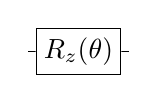
\begin{tikzpicture}
            \begin{yquant}
                qubit {} q[1];
                box {\(R_z(\theta)\)} q[0];
            \end{yquant}
        \end{tikzpicture}}} \\[1em]
        Faasinihe & \(P(\lambda)\) & \(
        \begin{pmatrix}
            1 & 0 \\
            0 & e^{i\lambda} \\
        \end{pmatrix}
        \) & \lower6pt\hbox{\yquantjoonis{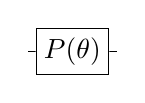
\begin{tikzpicture}
            \begin{yquant}
                qubit {} q[1];
                box {\(P(\theta)\)} q[0];
            \end{yquant}
        \end{tikzpicture}}} \\[1em]
        Juhitud eitus & \(\CNOT\) & \(
        \begin{pmatrix}
            1 & 0 & 0 & 0 \\
            0 & 0 & 0 & 1 \\
            0 & 0 & 1 & 0 \\
            0 & 1 & 0 & 0 \\
        \end{pmatrix}
        \) & \lower6pt\hbox{\yquantjoonis{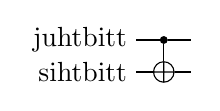
\begin{tikzpicture}
            \begin{yquant}
                qubit {juhtbitt} ctrl;
                qubit {sihtbitt} trgt;
                cnot trgt | ctrl;
            \end{yquant}
        \end{tikzpicture}}} \\
        Pauli \(X\) & \(X\) & \(
        \begin{pmatrix}
            0 & 1 \\
            1 & 0 \\
        \end{pmatrix}
        \) & \lower6pt\hbox{\yquantjoonis{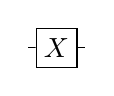
\begin{tikzpicture}
            \begin{yquant}
                qubit {} q[1];
                box {\(X\)} q[0];
            \end{yquant}
        \end{tikzpicture}}} \\[1em]
        Pauli \(Y\) & \(Y\) & \(
        \begin{pmatrix}
            0 & -i \\
            i & 0 \\
        \end{pmatrix}
        \) & \lower6pt\hbox{\yquantjoonis{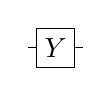
\begin{tikzpicture}
            \begin{yquant}
                qubit {} q[1];
                box {\(Y\)} q[0];
            \end{yquant}
        \end{tikzpicture}}} \\[1em]
        Pauli \(Z\) & \(Z\) & \(
        \begin{pmatrix}
            1 & 0 \\
            9 & -1 \\
        \end{pmatrix}
        \) & \lower6pt\hbox{\yquantjoonis{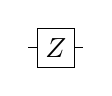
\begin{tikzpicture}
            \begin{yquant}
                qubit {} q[1];
                box {\(Z\)} q[0];
            \end{yquant}
        \end{tikzpicture}}} \\[1em]
        Hadamardi operaator & \(H\) & \(
        \frac{1}{\sqrt{2}} \begin{pmatrix}
            1 & 1 \\
            1 & -1 \\
        \end{pmatrix}
        \) & \lower6pt\hbox{\yquantjoonis{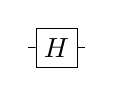
\begin{tikzpicture}
            \begin{yquant}
                qubit {} q[1];
                box {\(H\)} q[0];
            \end{yquant}
        \end{tikzpicture}}} \\[1em]
        Faasioperaator & \(S\) & \(
        \begin{pmatrix}
            1 & 0 \\
            0 & i \\
        \end{pmatrix}
        \) & \lower6pt\hbox{\yquantjoonis{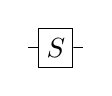
\begin{tikzpicture}
            \begin{yquant}
                qubit {} q[1];
                box {\(S\)} q[0];
            \end{yquant}
        \end{tikzpicture}}} \\[1em]
        Pöördfaasioperaator & \(S^{\dagger}\) & \(
        \begin{pmatrix}
            1 & 0 \\
            0 & -i \\
        \end{pmatrix}
        \) & \lower6pt\hbox{\yquantjoonis{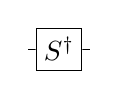
\begin{tikzpicture}
            \begin{yquant}
                qubit {} q[1];
                box {\(S^{\dagger}\)} q[0];
            \end{yquant}
        \end{tikzpicture}}} \\[1em]
        Bittide vahetus & \(\SWAP\) & \(
        \begin{pmatrix}
            1 & 0 & 0 & 0 \\
            0 & 0 & 1 & 0 \\
            0 & 1 & 0 & 0 \\
            0 & 0 & 0 & 1 \\
        \end{pmatrix}
        \) & \lower6pt\hbox{\yquantjoonis{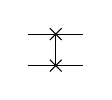
\begin{tikzpicture}
            \begin{yquant}
                qubit {} q[2];
                swap (q[0, 1]);
            \end{yquant}
        \end{tikzpicture}}} \\
        \midrule
        Mõõtmine & --- & --- & \lower6pt\hbox{\yquantjoonis{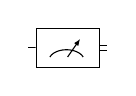
\begin{tikzpicture}
            \begin{yquant}
                qubit {} q[1];
                measure q[0];
            \end{yquant}
        \end{tikzpicture}}} \\
        \bottomrule
    \end{tabular}
    \caption{Töös kasutatud operaatorid, nende tähtistused, definitsioonid ja tähitused ahelas}
    \label{tab:gates}
\end{table}

Kvantäravate järjestuse ja bittidele rakendamise korra määrab kvantahel.
Joonis~\ref{fig:circuits} on näide ahelast. Igat üksikut biti või registrit
tervikuna tähistab horisontaalne traat. Traadist vasakul on sisend- ja paramal
väljundolekud, kui need on olulised. Operaatorid on kastid. Operaator rakendub
igale bitile, mille traat kasti läbib. Katsutid (punktiga lõppevad vertikaalsed
jooned) ühendavad operaatoreid juhtbitide või juhtregistritega, kui neid on.

\begin{figure}
    \centering
    \yquantjoonis{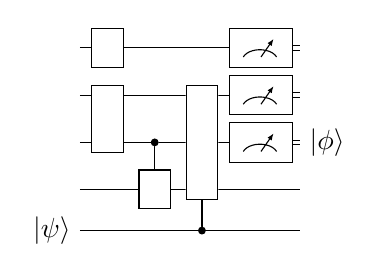
\begin{tikzpicture}
        \begin{yquant}
            qubit {} q[4];
            qubit {\(\ket{\psi}\)} q[+1];
            box {} q[0];
            box {} (q[1, 2]);
            box {} q[3] | q[2];
            box {} (q[1, 2, 3]) | q[4];
            measure q[0, 1, 2];
            output {\(\ket{\phi}\)} q[2];
        \end{yquant}
    \end{tikzpicture}}
    \caption{Kvantahela näide}
    \label{fig:circuits}
\end{figure}

Pikemalt tutvutavad ahelamudelit \cite{nielnsen+chuang} ja
\cite{kaye+laflamme+mosca}. Samas \cite{cao+etal} ja \cite{mcardle+etal} on
põgusamad tutvustused, kuid suunatud justnimelt kvantsimulatsioonile.


\subsection{LIITA EELMISEGA: Kvantarvutite eelis klassikaliste arvutite ees}

Mitmed olulised ülesanded on klassikaliselt praktiliselt lahenduvad vaid lihtsamatel juhtudel.
Kuulus näide on algarvuliste tegurite leidmise ülsanne, mille lahendamisalgoritmi keerukus on eksponetsiaalne: arvu suurenedes kulub tegurite leidmiseks eksponentsiaalselt rohkem mälu ja aega.
Kvantalgoritmi selle ülesande lahendamiseks leidis Shor~\cite{shot} ja tema algoritmi keerukus on kõigest polünoomne.
Seega võib kvantarvutitega olla võimalik lahendada ülesandeid, mille lahendamine klassikaliselt on põhimõtteliselt liiga kulukas~\cite{nielse+chuang, kaye+laflamme+mosca, cao+etal}.

Kvantalgorimtid saavad ära kasutada põimitust, mida klassikalises teoorias ei esine.
Samuti on kvantregistrisse võimalik talletada rohkem informatsiooni kui klassikalisse registrisse.
Uued vahendid teevadki võimalikuks uued algortmid~\cite{cao+etal}.

Ka faasi hindamine on üks nendest ülesannetest, mille lahendamine on kvantarvutuslikult soodsam.
Varsti näeme, et sellest tingituna on kvantarvutid sobivad elektronstruktuuri ülesande lahendamiseks, millega siin töös teglemegi~\cite{cao+etal, mcardle+etal}.

Ei saa mainimata jätta, et siiani pole kvantarvutuslikult olnud võimalik lahendada ühtegi ülesannet, mis on klassikaliselt lahendamiseks liiga raske.
Nimelt pole kvantarvutite riistvara selleks veel piisavalt arenenud.
Siiski on mõtet kvantalgortmide uurimisega tegeleda tuleviku tarvis.
Lähitulevikus võib õnnestuda ära kasutada hübriidalgoritme, mis kasutavad klassikalist ja kvantarvutit vaheldumisi~\cite{omalley+etal}.



\section{Faasi hindamise ALGORITM}\label{sec:pea}

See peatükk käsitleb faasi hindamise ülesannet ja selle rakendamist elektronstruktuuri ülesande lahendamiseks.

Jaotise~\ref{sec:qft} teemaks on kvantarvtuslik Fouirer' teisendus ja pöördteisendus, mis on vajalikud peatüki järgmises osas~\ref{sec:untiary}.

Jaotis~\ref{sec:unitary} käsitleb unitaarse operaatori omaväärtuste leidmist, milleks ongi faasi hindamise algoritm mõeldud.

Viimases jaotiseses~\ref{sec:hermit} näidatakse, kuidas faasi hindamise algoritmi on võimalik kasutada ka hermiitiliste (mitte tingimata unitaarsete) operaatorite omaväärtuste leidmiseks.
Arutlus viiakse läbi hamiltoniaani näitel, rõhutamaks faasi hindamise algoritmi kasulikkust elektronstruktuuri ülesande lahendamisel.


\subsection{Kvantarvutuslik Fourier' teisendus ja pöördteisendus}\label{sec:qft}

Kvantarvutusliku Fourier' teisenduse algoritm ja pöördteisenduse algoritm on faasi hindamise algoritmi tähtsad osad~\cite{nielsen+chuang, kaye+laflamme+mosca}.
Vaatame nende tööpõhimõtet.

Kvantarvtusliku Fourier' teisenduse mõju baasivektorile on
\begin{align}\label{f:qftdef}
    \QFT\colon
    \ket{j} \mapsto \frac{1}{\sqrt{2^n}} \sum_{k=0}^{2^n-1} e^{2\pi ijk/2^n} \ket{k} \rlap{,}
\end{align}
kus \(\ket{j}\) ja \(\ket{k}\) \(n\)-kvantbitised
baasivektorid~\cite{nielsen+chuang, kaye+laflamme+mosca}. Et tegemist on
lineaarse operatsiooniga, piisab vaadata mõju baasivektoritele.

\begin{figure}
    \centering
    \yquantjoonis{\begin{tikzpicture}[scale=0.8]
        \begin{yquant}
            qubit {\(\ket{j_1}\)} q[1];
            qubit {\(\ket{j_2}\)} q[+1];
            qubit {\(\vdots\)} q[+1]; discard q[2];
            qubit {\(\ket{j_{n-1}}\)} q[+1];
            qubit {\(\ket{j_n}\)} q[+1];
            h q[0];
            box {\(P(2\pi/2^2)\)} q[0] | q[1];
            text {\(\ \ldots\ \)} q[0, 1, 3, 4];
            h q[1];
            text {\(\ \ldots\ \)} q[0, 1, 3, 4];
            box {\(P(2\pi/2^{n-2})\)} q[1] | q[3];
            box {\(P(2\pi/2^{n-1})\)} q[1] | q[4];
            text {\(\ \ldots\ \)} q[0, 1, 3, 4];
            h q[3];
            box {\(P(2\pi/2^2\)} q[3] | q[4];
            h q[4];
            swap (q[0, 4]);
            swap (q[1, 3]);
            output {\(\frac{\ket0+e^{2\pi0.j_n}\ket1}{\sqrt{2}}\)} q[0];
            output {\(\frac{\ket0+e^{2\pi0.j_{n-1}j_n}\ket1}{\sqrt{2}}\)} q[1];
            output {\(\vdots\)} q[2];
            output {\(\frac{\ket0+e^{2\pi0.j_2\cdots j_n}\ket1}{\sqrt{2}}\)} q[3];
            output {\(\frac{\ket0+e^{2\pi0.j_1\cdots j_n}\ket1}{\sqrt{2}}\)} q[4];
        \end{yquant}
    \end{tikzpicture}}
    \caption{Kvantarvutusliku Fourier' teisneduse ahel~\cite{nielsen+chuang, kaye+laflamme+mosca}}
    \label{fig:qft}
\end{figure}

Näitame, et kvantarvutusliku Fourier' teisenduse realiseerib ahel joonisel~\ref{fig:qft}.

Kasutame tähistust, kus
\begin{multline}
    j_1j_2\cdots j_n.j_{n+1}j_{n+2}\cdots j_m \\
    = j_1 2^{n-1} j_2 2^{n-2} + \cdots + j_n 2^0 + j_{n+1} 2^{-1} j_{n+2} 2^{-2} + \cdots j_m 2^{-m} \rlap{,}
    \qquad j_i \in \{0, 1\} \rlap{.}
\end{multline}
NB! Selles ja järgmises jaotises on kõik komaga arvud kahendmurrud (mitte kümnendmurrud).

On vaja teada, et Hadamardi operaatori mõju baasvektoritele on
\begin{align}
    H\ket{0} = \frac{\ket{0} + \ket{1}}{\sqrt{2}}
\end{align}
ja
\begin{align}
    H\ket{1} = \frac{\ket{0} - \ket{1}}{\sqrt{2}} \rlap{.}
\end{align}
Viimased kaks tingimust saab kokku võtta üheks
\begin{align}
    H\ket{j_i} = \frac{\ket{0} + e^{2\pi i0.j_i}\ket{1}}{\sqrt{2}}\rlap{.}
\end{align}

Samuti on vaja teada, et parameetriga faasioperaatori mõju baasivektoritele on
\begin{align}
    P(\lambda)\ket{0} = \ket{0}
\end{align}
ja
\begin{align}
    P(\lambda)\ket{1} = e^{i\lambda}\ket{0} .
\end{align}
Viimasest kahest tingimusest järeldub kasulik omadus
\begin{align}\label{f:phase}
    P(2\pi i0.0j_2) = \frac{\ket{0} + e^{2\pi i 0.j_1} \ket{1}}{\sqrt{2}}
    = \frac{\ket{0}+e^{2\pi i0.j_1j_2}\ket{1}}{\sqrt{2}} .
\end{align}

Järgime joonise~\ref{fig:qft} ahela loogikat samm-sammult.

Algolek on
\begin{align}
    \ket{j_1} \otimes \ket{j_2} \otimes \cdots \otimes \ket{j_n} \rlap{.}
\end{align}

Kõigepealt tuleb esimesele kvantbitile mõjuda Hadamardi operaatoriga \(H\).
Pärast seda on olek
\begin{align}
    \frac{\ket{0} + e^{2\pi i0.j_1}\ket{1}}{\sqrt{2}} \otimes \ket{j_2} \otimes \cdots \otimes \ket{j_n} \rlap{.}
\end{align}

Järgmiseks tuleb mõjuda esimesele kvantbittile faasiväravaga \(P(2\pi/2^2)\) juhinduvalt teisest kvantbitist.
Kui \(j_2 = 0\), siis esimest bitti ei mõjutata, mis on sama hea, kui mõjuda operaatoriga \(P(2\pi 0.00)\).
Kui \(j_2 = 1\), siis mõjutakse operaatoriga \(P(2\pi 0.01)\).
Kokkuvõttes võib öelda, et teisele bitile mõjutakse operaatoriga \(P(2\pi 0.0j_2)\).
Tulenevalt valemist~\ref{f:phase} on pärast seda olek
\begin{align}
    \frac{\ket{0} + e^{2\pi i0.j_1j_2}\ket{1}}{\sqrt{2}} \otimes \ket{j_2} \otimes \cdots \otimes \ket{j_n} \rlap{.}
\end{align}

Edasi tuleb mõjuda esimesele kvantbitile faasiväravaga \(P(2\pi/2^3)\) juhinduvalt kolmandast kvantbitist.
Tulemuseks on
\begin{align}
    \frac{\ket{0} + e^{2\pi i0.j_1j_2j_3}\ket{1}}{\sqrt{2}} \otimes \ket{j_2} \otimes \cdots \otimes \ket{j_n} \rlap{.}
\end{align}

Sarnaselt tuleb toimida ka juhinduvalt ülejäänud kvantbititdest.
Lõpuks on tulemuseks
\begin{align}
    \frac{\ket{0} + e^{2\pi i0.j_1j_2\cdots j_n}\ket{1}}{\sqrt{2}} \otimes \ket{j_2} \otimes \cdots \otimes \ket{j_n} \rlap{.}
\end{align}

Järgmiseks, teise kvantbitiga tuleb toimida analoogselt esimesega.
Seejärel on olek
\begin{align}
    \frac{\ket{0} + e^{2\pi i0.j_1j_2\cdots j_n}\ket{1}}{\sqrt{2}}
    \otimes \frac{\ket{0} + e^{2\pi i0.j_2j_3\cdots j_n}\ket{1}}{\sqrt{2}}
    \otimes \ket{j_3} \otimes \cdots \otimes \ket{j_n} \rlap{.}
\end{align}

Kui sama skeemi järgida ülejäänud bitte jaoks, on lõpuks olek
\begin{align}
    \frac{\ket{0} + e^{2\pi i0.j_1j_2\cdots j_n}\ket{1}}{\sqrt{2}}
    \otimes \frac{\ket{0} + e^{2\pi i0.j_2j_3\cdots j_n}\ket{1}}{\sqrt{2}}
    \otimes \cdots
    \otimes \frac{\ket{0} + e^{2\pi i0.j_n}\ket{1}}{\sqrt{2}} \rlap{.}
\end{align}

Viimaks tuleb bittide järjekorda vahetada, mida on joonise~\ref{fig:qft} ahelas tehtiud \(\SWAP\)-väravaga.
Peala seda on olek
\begin{align}\label{f:qftfinal}
    \frac{\ket{0} + e^{2\pi i0.j_n}\ket{1}}{\sqrt{2}}
    \otimes \frac{\ket{0} + e^{2\pi i0.j_{n-1}j_n}}{\sqrt{2}}
    \otimes \cdots
    \otimes \frac{\ket{0} + e^{2\pi i0.j_1j_2\cdots j_n}\ket{1}}{\sqrt{2}} \rlap{.}
\end{align}

Avades sulud ja koondades, saab oleku~\ref{f:qftfinal} kirja panna kujul
\begin{equation}\label{f:qftfinaltrans}
    \frac{1}{\sqrt{2^n}}\sum_{k=0}2^{n-1}e^{2\pi ijk/2^n}\ket k \rlap{,}
\end{equation}
milline peabki olema Fourier' teisenduse tulemus~\cite{nielsen+chuang, kaye+laflamme+mosca}.

Järgnevas jaotises läheb vaja ka kvantarvutusliku Fourier' pöördteisendust, mille kohaselt
\begin{align}
    \QFT^{-1}\colon
    \frac{1}{\sqrt{2^n}} \sum_{k=0}^{2^n-1} e^{2\pi ijk/2^n} \ket{k} \mapsto \ket{j} \rlap{.}
\end{align}
Pöörteisenduse ahela saamiseks tuleb teisenduse ahel pöörata: ahel tuleb koostada vastupidises järjekorras, asendades operaatorid pöördoperaatoritega~\cite{kaye+laflamme+mosca}.
Kehtivad seosed
\begin{align}\label{f:iqftdef}
    H &= H^{\dagger} \rlap{,} \\
    P(-\lambda) &= P^{\dagger}(\lambda) \rlap{,} \\
    \SWAP &= \SWAP^{\dagger} \rlap{.}
\end{align}

Klassikalise Fourier' teisenduse valem on
\begin{align}\label{f:cftdef}
    y_k = \frac{1}{\sqrt{N}} \sum_{j=0}^{N-1}e^{2\pi ijk/N} x_j \rlap{.}
\end{align}
Valemite \ref{f:qftdef} ja \ref{f:cftdef} võrdlusest selgub, et kvantarvutusliku Fourier' teisenduse käigus toimub klassikaline Fourier' teisendus, kui võtta \(N = 2^n\)~\cite{nielsen+chuang}.

Klassikaliselt kulub Fourier' teisenduse läbi viimiseks \(N \log{N}=n 2^n \) sammu, kvantavutuslikult vaid \(\log^2{N} = n^2\) sammu.
Pealt näha on antud ülesande lahendamine kvantarvutuslikult oluliselt efektiivsem kui klassikaliselt~\cite{nielsen+chuang}.

Paraku talletub Fourier' teisenduse tulemus kvantarvutusliku Fourier' teisenduse käigus lõppoleku amplituudidesse ja pole seega otseselt mõõdetav~\cite{nielnse+chuang}.
Sellest tulenevalt ei saa kvantarvutusliku Fourier' teisendust kasutada lihtsalt klassikalise Fourier' teisenduse kiiremaks läbiviimiseks.


Siiski õnnestub kvantarvtusliku Fourier' teisendust kasutada teatud ülesannete klassikalisest efektiivsemaks lahendamiseks.
Antud töö jaoks on oluline, et see leiab kasutust faasi hindamise algoritmis, mida tutvustab järgmine jaotis.


\subsection{Unitaarse operaatori omaväärtusülesanne}\label{sec:unitary}

Unitaarse operaatori \(U\) jaoks kehtib omaväärtusvõrrand
\begin{align}\label{f:eigen}
    U \ket{u} = e^{2\pi i\phi} \ket{u}\rlap{,}
\end{align}
kus \(\ket{u}\) on \(U\) omavektor ja \(e^{2\pi i\phi}\) omaväärtus.
Faasi hindamise ülesandes on eesmärgiks leida unitaarse operaatori omaväärtus, mida kutsutakse ka selle operaatori faasiks.

Valemis~\ref{f:eigen} on faas on määratud suurusega \(\phi \in [0, 1)\).
Näitame, et \(\phi\) leidmiseks sobib ahel joonisel~\ref{fig:pea}.

\begin{figure}[h]
    \centering
    \begin{tikzpicture}
        \begin{yquant}
            qubit {$\ket0$} pea[1];
            qubit {$\ket0$} pea[+1];
            qubit {$\vdots$} pea[+1]; discard pea[2];
            qubit {$\ket0$} pea[+1];
            qubit {$\ket0$} pea[+1];
            qubit {$\ket u$} state;
            box {$\mathop{\rm QFT}$} (pea[0], pea[1], pea[2], pea[3], pea[4]);
            box {$U^{2^0}$} state | pea[4];
            box {$U^{2^1}$} state | pea[3];
            text {$\ \ldots\ $} pea[0], pea[1], pea[3], pea[4], state;
            box {$U^{2^{n-2}}$} state | pea[1];
            box {$U^{2^{n-1}}$} state | pea[0];
            box {$\mathop{\rm QFT}\nolimits^{-1}$} (pea[0], pea[1], pea[2], pea[3], pea[4]);
            measure pea[0], pea[1], pea[3], pea[4];
            output {$\phi_1$} pea[0];
            output {$\phi_2$} pea[1];
            output {$\vdots$} pea[2];
            output {$\phi_{n-1}$} pea[3];
            output {$\phi_n$} pea[4];
            output {$\ket u$} state;
        \end{yquant}
        \end{tikzpicture}
    \caption{Kvantahel \(U\) faasi hindamiseks \cite{nielnse+chuang, kaye+laflamme+mosca}}
    \label{fig:pea}
\end{figure}

Joonise~\ref{fig:pea} ahelas on kaks kvantregistrit.
Faasi hindamise registrit kujutavad ülemised \(n\) traati.
Kõige alumine traat on olekuregister.%
\footnote{Kuigi olekuregistrit on kujutatud vaid ühe traadiga, võib selles olla kuitahas palju kvantbitte.}

Järgime joonise~\ref{fig:pea} ahela loogikat samm-sammult.

Joonisel~\ref{fig:pea} on eeldatud, et olekuregister on juba \(U\) omaolekus
\(\ket{u}\), praktikas tuleb see olek kuidagi prepareerida.

Esimese sisulise sammuna tuleb faasi hindamise registrile mõjuda kvantarvutusliku Fourier' teisenduse väravaga.%
\footnote{Kvantarvutuslku Fourier' teisenduse värava realiseerimist kvantahalana käsitles eelmine jaotis~\ref{sec:qft}.}
Kui eeldada, et faasi hindamise registri kvantbitid olid enne kõik olekus \(\ket{0}\), siis on kvantarvutusliku Fourier' teisenduse tulemuseks olek
\begin{align}\label{f:peainit}
    \underbrace{\frac{\ket{0}+\ket{1}}{\sqrt{2}}
    \otimes \cdots
    \otimes \frac{\ket{0}+\ket{1}}{\sqrt{2}}}_n
    \otimes \ket{u} \rlap{.}
\end{align}

Järgmisena tuleb olekuregistile mõjuda operaatoriga \(U^{2^0}\) juhinduvalt faasi hindasmie registri viimasest bitist.
Selle tulemuseks on olek
\begin{align}\label{f:peau0}
    \underbrace{\frac{\ket{0}+\ket{1}}{\sqrt{2}}
    \otimes \cdots
    \otimes \frac{\ket{0}+\ket{1}}{\sqrt{2}}}_{n - 1}
    \otimes \frac{\ket{0}+e^{2\pi i2^0\phi}\ket{1}}{\sqrt{2}}
    \otimes \ket{u} \rlap{.}
\end{align}

Veendume selles võttes \(\ket{u} = \alpha\ket{0} + \beta\ket{1}\).
Siis oleku~\ref{f:peainit} saab kirja panna kujul
\begin{multline}
    \underbrace{\frac{\ket{0}+\ket{1}}{\sqrt{2}}
    \otimes \cdots
    \otimes \frac{\ket{0}+\ket{1}}{\sqrt{2}}}_n
    \otimes \paren{\alpha \ket{0} + \beta \ket{1}} \\
    = \underbrace{\frac{\ket{0}+\ket{1}}{\sqrt{2}}
    \otimes \cdots
    \otimes \frac{\ket{0}+\ket{1}}{\sqrt{2}}}_{n - 1}
    \otimes \frac{1}{\sqrt{2}} \paren{
        \alpha \ket{00} + \alpha \ket{10}
        + \beta \ket{01} + \beta \ket{11}
    } \rlap{.}
\end{multline}
Uus olek on
\begin{multline}
    \underbrace{\frac{\ket{0}+\ket{1}}{\sqrt{2}}
    \otimes \cdots
    \otimes \frac{\ket{0}+\ket{1}}{\sqrt{2}}}_{n - 1}
    \otimes \frac{1}{\sqrt{2}} \paren{
        \alpha \ket{00} + \alpha U^{2^0} \ket{10}
        + \beta \ket{01} + \beta U^{2^0} \ket{11}
    } \\
    = \underbrace{\frac{\ket{0}+\ket{1}}{\sqrt{2}}
    \otimes \cdots
    \otimes \frac{\ket{0}+\ket{1}}{\sqrt{2}}}_{n - 1}
    \otimes \frac{1}{\sqrt{2}} \paren{
        \alpha \ket{00} + \alpha e^{2\pi i2^0\phi} \ket{10}
        + \beta \ket{01} + \beta e^{2\pi i2^0\phi} \ket{11}
    } \\
    = \underbrace{\frac{\ket{0}+\ket{1}}{\sqrt{2}}
    \otimes \cdots
    \otimes \frac{\ket{0}+\ket{1}}{\sqrt{2}}}_{n - 1}
    \otimes \frac{\ket{0} + e^{2\pi i\phi 2^0} \ket{1}}{\sqrt{2}}
    \otimes \paren{\alpha \ket{0} + \beta \ket{1}} \rlap{,}
\end{multline}
mis ongi olek~\ref{f:peau0}.

Edasi tuleb olekuregistrile mõjuda operaatoriga \(U^{2^1}\) juhinduvalt faasi hindamise registri eelviimasest bitist.
Peale seda on olek
\begin{align}
    \underbrace{\frac{\ket{0} + \ket{1}}{\sqrt{2}}
    \otimes \cdots
    \otimes \frac{\ket{0} + \ket{1}}{\sqrt{2}}
    }_{n-2}
    \otimes \frac{\ket{0} + e^{2\pi i2^1\phi} \ket{1}}{\sqrt{2}}
    \otimes \frac{\ket{0} + e^{2\pi i2^0\phi} \ket{1}}{\sqrt{2}}
    \otimes \ket{u} \rlap{.}
\end{align}

Sama skeemi järgi tuleb jätkata.
Lõpuks on tulemuseks
\begin{align}\label{f:peauend}
    \frac{\ket{0}+ e^{2\pi i2^{n-1}\phi}}{\sqrt{2}}
    \otimes \frac{\ket{0}+ e^{2\pi i2^{n-2}\phi}}{\sqrt{2}}
    \otimes\cdots
    \otimes \frac{\ket{0}+ e^{2\pi i2^0\phi}}{\sqrt{2}}
    \otimes\ket{u}
\end{align}

Kui tähistada \(\phi=0.\phi_1\phi_2\cdots\phi_n\), siis võtab olek~\ref{f:peauend} kuju
\begin{align}
    \frac{\ket{0}+ e^{2\pi i0.\phi_n}\ket{1}}{\sqrt{2}}
    \otimes \frac{\ket{0}+ e^{2\pi i0.\phi_{n-1}\phi_n}\ket{1}}{\sqrt{2}}
    \otimes\cdots
    \otimes \frac{\ket{0}+ e^{2\pi i0.\phi_1\phi_2\cdots\phi_n}\ket{1}}{\sqrt{2}}
    \otimes\ket{u} \rlap{,}
\end{align}
sest
\begin{align}
    e^{2\pi i2^m\phi}
    = e^{2\pi i2^m 0.\phi_1\phi_2\cdots\phi_n}
    = e^{2\pi i0.\phi_m\phi_{m+1}\cdots\phi_n} \rlap{,}
\end{align}
globaalse faasi täpsusega.

Lõpuks tuleb faasi hindamise registrile mõjuda kvantarvutusliku Fourier' pöördteisendse väravaga.
Valemite~\ref{f:qftfinal}, \ref{f:qftfinaltrans} ja \ref{f:iqftdef} põhjal on tulemuseks
\begin{align}\label{f:peafinal}
    \ket{\phi_1} \otimes \ket{\phi_2} \otimes \cdots \otimes \ket{\phi_n} \otimes \ket{u} \rlap{.}
\end{align}

Kui süsteem on olekus~\ref{f:peafinal}, siis faasi hindamise registri mõõtmine annab tulemuseks klassikaliste bittide jada
\begin{align}
    \phi_1, \phi_2, \cdots, \phi_n \rlap{,}
\end{align}
millega on \(\phi = 0.\phi_1\phi_2 \cdots \phi_n\) määratud.

Äsja arutlesime eeldusel, et faasi hindamise registris on sama palju bitte \(n\), kui on vaja \(\phi = 0.\phi_1\phi_2 \cdots \phi_m\) esitamiseks kahendsüsteemis \(m = n\).
Praktilisel kaalutlustel ei pruugi see nii olla: \(m\) väärtus ei ole ette teada, faasi hindamiseks on kasutada piiratud arv bitte \(n < m\).

Kui \(n > m\), jääb eelnenud arutelu kehtima, ainult et \(\phi_{m+1}, \phi_{m+2}, \phi_n = 0\).

Saab näidata, et juhul, kui \(n < m\), on suurima mõõtmistõenõosusega tulemuseks \(\phi\) hinnang \(n\)-bitise täpsusega~\cite{kaye+laflamme+mosca}.
Suurima tõenõosusega kehtib
\begin{equation}
    0.\phi_1\phi_2\cdots\phi_n \in [\phi - 2^{-n-1}, \phi + 2^{n+1}] \rlap{.}
\end{equation}
Seega antud skeemi saab kasutada ka juhul, kui \(m\) pole ette teada või \(n\) on piiratud.
Mõõtmis\-tulemuste seast tuleb valida kõige tõenõolisem tulemus.

Faasi hindamise algoritm on osa Shori algoritmist algarvuliste tegurite leidmiseks, mis on oluline, sest Shori algoritmi keerukus on kõigest polünoomne, võrreldes sama eesmärgi jaoks parima klassikalise algoritmiga, mille keerukus on eksponentsiaalne~\cite{cao+etal, kaye+laflamme+mosca}.
Niisiis faasi hindamise algoritm võimalab mõnesid ülesandeid klassikalisest efektiivsemalt lahendada.

Antud töös kastuame faasi hindamise algoritmi hamiltoniaani omaväärtuste leidmiseks, mis on elektronstruktuuri ülesande lahendamise kulukas osa ja mida käsitleb järmgine jaotis.


\subsection{Hermiitilise operaatori omaväärtusülesanne}\label{sec:hermit}

Elektronstruktuuri ülesande lahendamiseks tuleks leida hamiltoniaani omaväärutused.
Eelmises jaotises~\ref{sec:unitary} selgus, et faasi hindamise algoritmi kasutades saab leida unitaarse operaatori omaväärtused, kuid hamiltoniaan pole enamasti unitaarne.
Osutub, et faasi hindamise algoritmi abil on siiski võimalik leida ka hermiitilise operaatori omaväärtused.
Näitame sedas keskendudes hamiltoniaanile.

Ajalise arengu operaator on
\begin{align}
    U = e^{-iHt} \rlap{,}
\end{align}
kus \(H\) on algne hamiltoniaan ja \(t\) skaleerimiskonstant, mille valikus leppime kokku hiljem.
Kuna hermiitilise operaatori eksponent on alati unitaarne, siis \(U\) on unitaarne.

Operaatori spektraallahutuse põhjal defineeritakse operaatori funktsioon.
Antud juhul on \(U=U(H)\).
Kui \(\ket{E_n}\) on \(H\) omavektor, siis kehtib
\begin{align}\label{f:eigenhermit}
    U \ket{E_n} = e^{-iHt}\ket{E_n} = e^{-i E_n t} \ket{E_n} \rlap{,}
\end{align}
kus \(E_n\) on \(H\) omaväärtus.

Samas eelmise jaotise~\ref{sec:unitary} põhjal oskame leida \(\phi\) nii, et
\begin{align}\label{f:eigenunitary}
    U \ket{u} = e^{2\pi i\phi} \rlap{.}
\end{align}

Valemite~\ref{f:eigenhermit} ja~\ref{f:eigenunitary} võrdlusest selgub, et leidnud \(\phi\) on võimalik arvutada
\begin{align}
    E_n = -\frac{2\pi\phi}{t} \rlap{,}
\end{align}
mis oligi meie eesmärk.

Et \(\phi \in [0, 1)\), siis peab lisaks kehtima
\begin{align}
    -\frac{E_n t}{2\pi} \in [0, 1) \rlap{.}
\end{align}
mis seab piirangud \(t\) valmiseks~\cite{whitfield+etal}.

Skaleerimiskonstanti \(t\) valimiseks on mitu võimalust.

Selles töös on tehtud valik
\begin{align}
    t = -\frac{2\pi}{2E_\mathrm{t}} \rlap{,}
\end{align}
kus \(E_t \ge \abs{E_n}\) on energia tõke, mida on vaja eelnevalt teada.
Arvestades faasi perioodilisust kehtib siis
\begin{align}
    E_n = \begin{cases}
        -\frac{2\pi\phi}{2E_t}\rlap{,} & \text{kui } \phi < \frac{1}{2} \\
        E_t - \frac{2\pi\phi}{2E_t}\rlap{,} & \text{kui } \phi \ge \frac{1}{2} \\
    \end{cases}
\end{align}

Oleme näidanud, et faasi hindamise algoritm sobib hamiltoniaani omaväärtuste leidmiseks.
Eelduseks on Focki ruumi hamiltoniaani estiamine kvanatahelana.

Oluline on et, faasi hindamsie algoritm on klassikalistest algoritmidest efektiivsem, sest omaväärtuste leidmine ongi elektronstruktuuri ülesande lahendamise üks kulukaim etapp.
Seega loodetakse faasi hindamise algoritmiga lahendada keerulisemaid ülesandeid, kui on võimalik klassikaliset~\cite{mcardle+etal, cao+etal}.

Siin esitatud skeemi täiendavaks eeliseks on, et näiteks põhienergia leidmiseks pole vaja teada põhioleku vektori täpset kuju.
Hatree-Focki hinnang võib olla piisav.
Kui kehtib
\begin{align}
    \ket{\text{HF}} = \sum_n \alpha_i \ket{E_i} \rlap{,}
    \qquad \alpha_i > \alpha_2, \alpha_3, \ldots, \alpha_n
\end{align}
siis on tagatud, et suurima tõenäosusega mõõtmistulemus on põhineriga \(E_1\) hinnang~\cite{whitfield+etal}.


\section{Hamiltoniaani SIMULEERIMINE}\label{sec:qcirc}

Selles peatkükis leiame kvantahela hamiltoniaani simuleerimiseks.


\section{Jordan-Wigneri teisendus}\label{sec:jw}

Järgmise peatükki tarvis on vajalik kvantahelana realiseerida unitaarset operaatorit
\begin{equation}\label{eq:hamtime}
  U = e^{-iHt}\rlap{,}
\end{equation}
kus \(H\) on hamiltoniaan.
Varasemalt käsitlesime hamiltoniaani \(H\) Focki ruumi operaatorina.
Eelmistes peatükkides oli hamiltoniaan \(H\) Focki ruum objekt.
Selle realiseerimiseks kvantahelana viimes slles peatükis läbi Jordan-Wigneri teisenduse~\cite{jordan+wigner}, mis viib hamiltoniaani üle kvantbittide ruumi.

Siin töös me Jordan-Wigneri teisenduse üksikasju ei käsitle, kuid toome ära mõned selle kasulikud omadused.

Esiteks, selle teisenduse tulemusena saame hamiltoniaani \(H\) Pauli sõnede summana~\cite{whitfield+etal}.
Pauli sõnede all mõistame Pauli maatriksite tensorkorrutisi.
Sümboolselt
\begin{equation}\label{eq:paulisum} H = \sum_i h_i\rlap{,} \end{equation}
kus $h_i$ on Pauli sõne.

Edaspidi tähistame Pauli sõnesesid lühidalt
\begin{equation} h_i=P_{j_1}P_{j_2}\cdots P_{j_k} \rlap{,}\end{equation}
kus \(j_1\), \(j_2\), $\ldots$, \(j_k\) tähistavad kvantbitte, millele \(P_{j_1}\), \(P_{j_2}\), \(\ldots\), \(P_{j_k}\in\{X,Y,Z\}\) mõjuvad.
Näiteks \(X_1Y_2Z_4=X\otimes Y\otimes 1\otimes Z.\)
(Selles tähistuses peab Pauli sõne dimensioon olema selge kontekstist, sest viimase Pauli X-, Y- või Z-maatrikisi järel võib olla kuitahes palju ühikmaatrikseid.)

Teiseks, võimalikele puhastele olekutele vastavad vektorid kujul
\begin{equation}
  \ket{x_1x_2\cdots x_n}
     = \ket{x_1}\otimes\ket{x_2}\otimes\cdots\otimes\ket{x_n}\rlap{,}
\end{equation}
kus $x_1$, $x_2$, $\ldots$ $x_n\in\{0,1\}$ näitab spinnorbitaalide $1$, $2$, $\ldots$, $n$ täidetust ja $n$ on spinnorbitaalide arv süsteemis~[viide?].
Näiteks, kvantbittide ruumi seisund \(\ket{\Psi_0}=\ket{1100}\) vastab Focki ruumi seisundile, kus alumised kaks spinnorbitaali on täidetud ja ülemised kaks mitte~\cite{szabo+ostlund, mcardle+etal}.


\subsection{Pauli $Z$ maatriksite tensorkorrutise eksponent}

Soovime kvantahelana realiseerida operaatorit~\ref{eq:hamtime}.
Vaatame kõigepealt lihtsat juhtu.
Kui
\begin{equation}
  H=Z_{j_1}Z_{j_2}\cdots Z_{j_n}\rlap{,}
\end{equation}
siis operaatorit~\ref{eq:hamtime} realiseerib kvantahel joonisel~\ref{f:expz}.

\begin{figure}[h]
  \centering
  \yquantjoonis{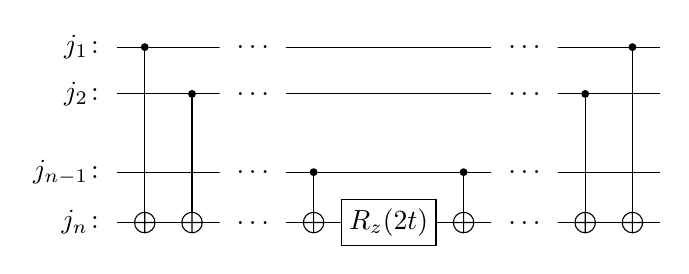
\begin{tikzpicture}
    \begin{yquant}
      qubit {$j_1\colon$} q[1];
      qubit {$j_2\colon$} q[+1];
      qubit {} q[+1]; discard q[2];
      qubit {$j_{n-1}\colon$} q[+1];
      qubit {$j_n\colon$} q[+1];
      cnot q[4] | q[0];
      cnot q[4] | q[1];
      text {$\ \ldots\ $} q[0,1,3,4];
      cnot q[4] | q[3];
      box {$R_z(2t)$} q[4];
      cnot q[4] | q[3];
      text {$\ \ldots\ $} q[0,1,3,4];
      cnot q[4] | q[1];
      cnot q[4] | q[0];
    \end{yquant}
  \end{tikzpicture}}
  \caption{Operaatori \(e^{-iZ_{j_1}Z_{j_2}\cdots Z_{j_n}t}\) realiseerimine kvantahelana. Bitte, mis \(j_1\), \(j_2\), \(\cdots\), \(j_n\) hulgas ei esine, pole näidatud}
  \label{f:expz}
\end{figure}

Teisisõnu, bitile \(j_n\) tuleb järjest rakenda bittide \(j_1\), \(j_2\), \(\cdots\), \(j_{n-1}\) juhitud \(\cnot\)-väravavaid.
Siis tuleb bitti \(j_n\) pöörata väravaga \(R_z(2a)\).
Viimaks tuleb bitile \(j_n\) järjest rakendada bittide \(j_{n-1}\), \(j_{n-2}\), \(\cdots\), \(j_1\) jihtud \(\cnot\)-väravaid.
Bitte, mis \(j_1\), \(j_2\), \(\cdots\), \(j_n\) hulgas ei esine, ei mõjutata~\cite{mansky+etal}.

Kesksele väravale \(R_z(2a)\) eelnev \(\cnot\)-väravate osa arvutab bitide \(j_1\), \(j_2\), \(\cdots\), \(j_n\) paarsuse.
Keskne värav \(R_z(2a)\) teeb sobiva pöörde.
Järgnev \(\cnot\)-väravate osa kustutab ära nüüdseks ebavajaliku informatsiooni paarsuse kohta~\cite{nielsen+chuang}.


\subsection{Pauli $X$, $Y$ ja $Z$ maatriksite tensorkorrutise eksponent}

Vaatame nüüd keerukamat juhtu, kus \(H\) on Pauli X-, Y- ja Z-maatriksite tensorkorrutis, mitte vaid Z-maatriksite tensorkorrutis.
Näiteks, olgu
\begin{equation}
  H=Z_1X_2Y_3\rlap{.}
\end{equation}

Ahela koostamiseks kasutame ära asjaolu, et
\begin{equation} Z=HXH \end{equation}
ja
\begin{equation} Z=S^{\dagger}HYHS\rlap{.} \end{equation}
Järeldame, et \(e^{-iZ_1X_2Y_3}\) ahel on võimalik saada \(e^{-iZ_1Z_2Z_3}\) ahelast sobivate baasiteisendustega.
Sobiv ahel on joonisel~\ref{f:zxyex}~\cite{nielsen+chuang}.

\begin{figure}[h]
  \centering
  \yquant{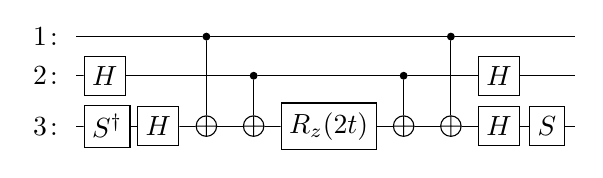
\begin{tikzpicture}
    \begin{yquant}
      qubit {$1\colon$} q[1];
      qubit {$2\colon$} q[+1];
      qubit {$3\colon$} q[+1];
      box {$H$} q[1];
      box {$S^{\dagger}$} q[2];
      box {$H$} q[2];
      cnot q[2] | q[0];
      cnot q[2] | q[1];
      box {$R_z(2t)$} q[2];
      cnot q[2] | q[1];
      cnot q[2] | q[0];
      box {$H$} q[1];
      box {$H$} q[2];
      box {$S$} q[2];
    \end{yquant}
  \end{tikzpicture}}
  \caption{\(e^{-iZ_1X_2Y_3}\) realiseerimine kvantahelana}
  \label{f:zxyex}
\end{figure}


\subsection{Pauli sõnede summade eksponent}

Üldjuhul on hamiltoniaan Pauli sõnede summa~\ref{eq:paulisum}.
Kui summa liikmed kommuteeruvad, siis võime kirjutada
\begin{equation}
  e^{-i\sum_i h_it}=\prod_ie^{-ih_it}\rlap{,}
\end{equation}
enamasti see aga nii ei ole.

On näidatud, et
\begin{equation}
  e^{-i\sum_i h_it}=\lim_{\Delta t\rightarrow0}\paren{\prod e^{-ih_i t/\Delta t}}^{\Delta t}
\end{equation}
ka mittekommuteeruvate summa liikmete $h_i$ puhul.
Seega lõpliku $\Delta t$ puhul
\begin{equation}
  e^{-i\sum_i h_it}\approx\paren{\prod e^{-ih_i t/\Delta t}}^{\Delta t}\rlap{,}
\end{equation}
kus paras $\Delta t$ väärtus tuleb enamasti leida eksperimentaalselt.
Seda meetodit ahela koostamiseks nimetatakse Suzuki-Trotteri lahutuseks või lihtsalt trotteriseerimiseks~\cite{mansky+etal}



\chapter{Metoodika}\label{chap:methods}

Selles peatükis võtame kokku protseduuri molekuli põhienergia leidmiseks.
Samuti tutvustame vahendeid arvutuste läbiviimiseks.


\section{Lahendamise skeem}

Esitame nüüd molekulaarse hamiltonaani energia leidmise sammud.

Ülesande lahendamine algab molekuli geomeetria kirja panemisest.
Tuleb määrata aatomite koosseis molekulis ja aatomite vahelised kaugused.
Samuti tuleb valida keemiline baas.
Sealt edasi saab leida konkreetse molekuli hamiltoniaani kuju.
Hamiltoniaani tuleb seejärel lihtsustada Born-Oppenheimeri ja Hatree-Focki lähenduses.
Lõpuks tuleb hamiltonaain esitada teise kvantiseerimise kujul.

Samuti tuleb leida huvipakkuvale olekule võimalikult lähedane olek Hartree korrutisena.

Järgmisena tuleb Focki ruumi hamiltoniaan esitada kvantbittide ruumis.
Selleks saab kasutada Jordan-Wigneri teisendust.
Järgmiseks tuleb kvantahelana realiseerida operaator, mis on hamiltoniaani eksponent.
Et hamiltoniaan on pärast Jordan-Wigneri teisendust Pauli sõnede summa, siis leidub skeem selle esitamiseks kvantahalana, kuid seda võib olla vaja trotteriseerida.

Faasihindamise jaoks on oluline, et unitaarne operaator oleks juhitud.
Juhitud unitaarse operaatori saab kui kvantahelas asendada kõik pöörded juhitud pööretega.
Nõnda toiminud, sõltub iga Pauli sõne rakendamine sellest, mis on juhtkvantbiti olek.
Kui juhtkvantbitt on olekus \(\ket0\), pööre ei rakendu.
Et paarsuse arvutamine ja selle tagasi panemine on pöördoperatsioonid, siis kokkuvõttes antud Pauli sõne justkui ei rakendu.
Kui juhtkvantvitt on olekus \(\ket1\) pööre rakendub ja rakendub ka Pauli sõne tervikuna.

Eraldi tuleb arvestada hamiltoniaani seda liiget, mis on ühikmaatriksite tensorkorrutis.
Sellise liikme eksponent on globaalse faasi operaator, mille juhtimiseta juhul võib jätta arvestamata.
Samas juhitud globaalse faasi operaator rakendaine muudab suhtelise faasi ja seda peab arvestama.
Juhtitud globaalse faasi operaatori võib asendanda juhtkvantvitil rakendatud suhtelise faasi opetaatoriga, nagu näha joonisel~\ref{fig:globphase}.

\begin{figure}[h]
    \centering
    \yquantjoonis{\begin{tikzpicture}
        \begin{yquantgroup}
            \registers{
                qubit {} q[2];
            }
            \circuit{
                box {\(GP(\alpha)\)} q[1] | q[0];
            }
            \equals
            \circuit{
                box {\(P(-\alpha)\)} q[0];
            }
        \end{yquantgroup}
    \end{tikzpicture}}
    \caption{Juhitud globaalse faasi operaaotri saab asendada juhtkvantbitile rakendatud faasi operaatoriga, mille argument peab olema vastupidine~\cite{nielsen+chuang}}
    \label{fig:globphase}
    \TODO{Üks traat on puudu}
\end{figure}


Viimaks tuleb koostada faasi hindamise kvantahel ja seda käitada.
Trotteriseerimise sammude arv ja faasi hindamise registri suurus tuleb valida sobivalt.

\TODO{Kas siin peaks olema lahendamise skeem joonisena?}


\section{Kasutatud vahendid}

Töös kasutsime programmeerimiskeelt Python.

Geomeetriast hamiltonaani saamist ja Jordan-Wigneri teisendust võimaldas teek OpenFermion~\cite{openfermion}.

Kvantahela koostamiseks ja selle klassikaliseks simuleerimiseks kasutasime teeki Qiskit~\cite{qiskit}.

Trotterisammude arvu, faasi hindamise registri suuruse ja energia piirväärtuse valikut selgitab järgmine peatükk.
Keemiliseks baasiks võtsime STO-3G.


\chapter{Tulemused}\label{chap:results}


\section{Vesiniku molekuli energia}

Selles töös võtsime mudelsüsteemiks \(\mathrm{H}_2\) molekuli.
STO-3G baasis on selle molekuli hamiltoniaan neljakvantbitine.

\begin{figure}[h]
    \centering
    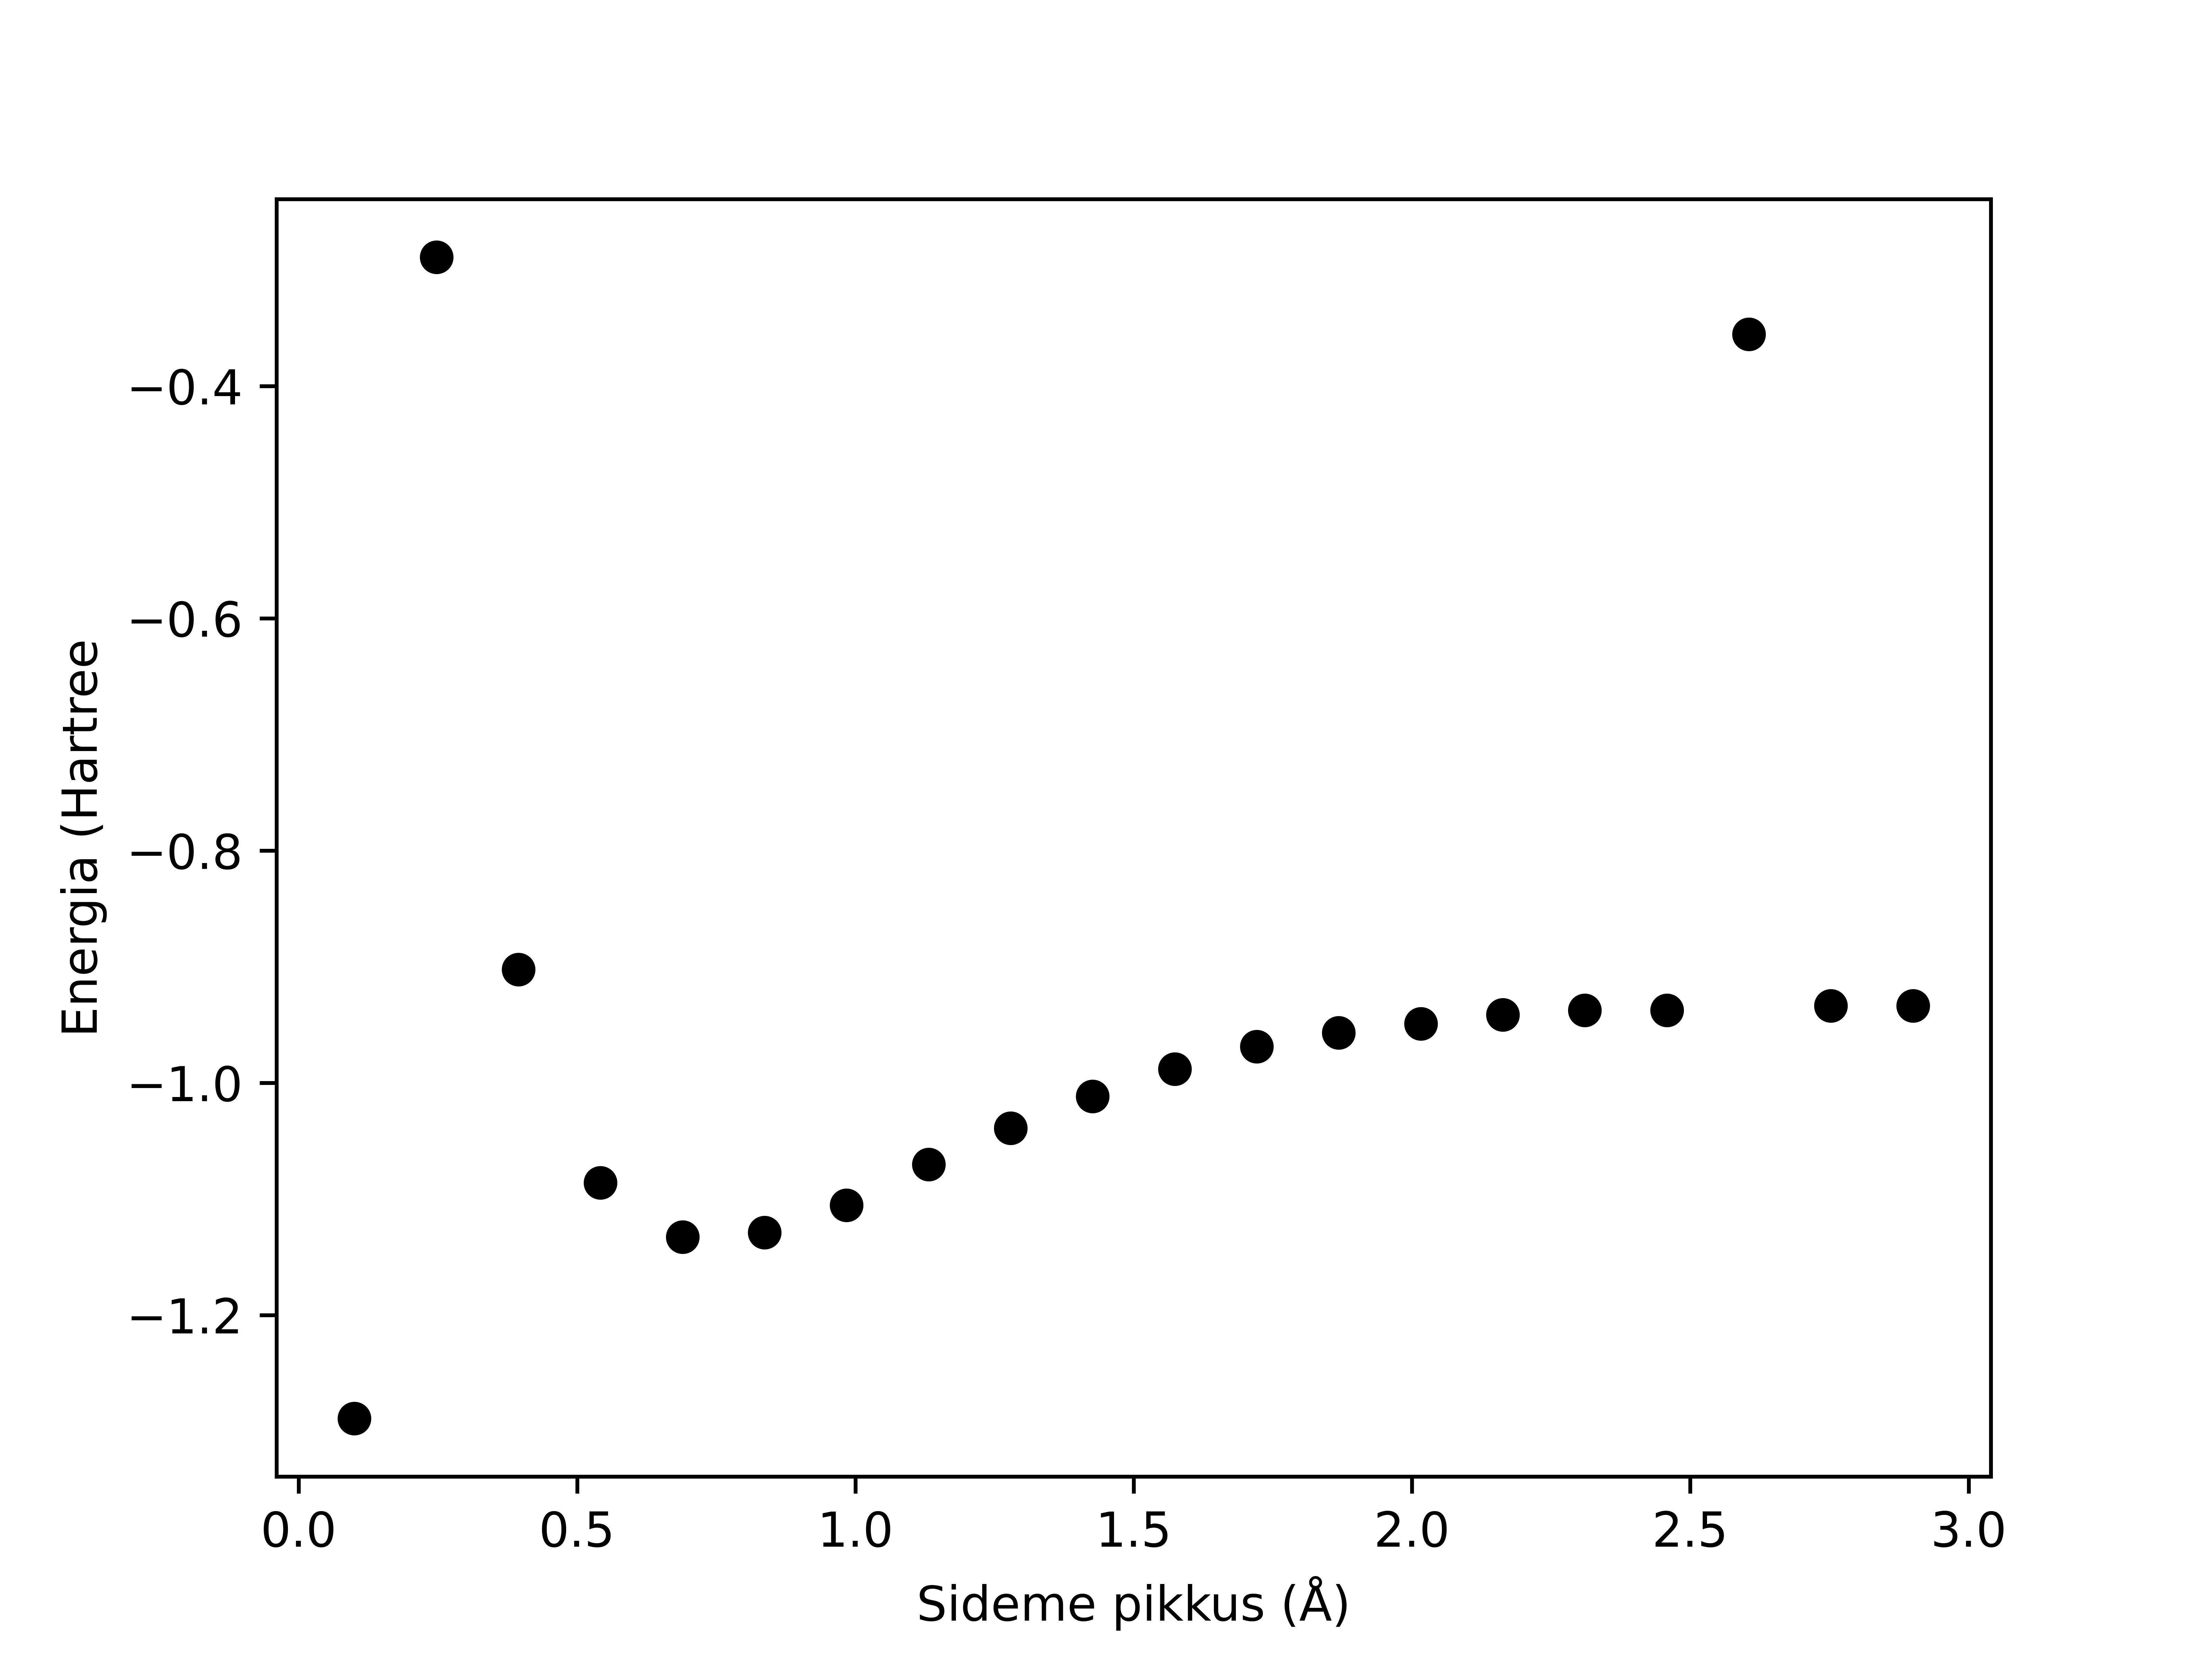
\includegraphics{scan.jpg}
    \caption{Vesiniku elektronkatte energia sõltuvus sideme pikkusest}
    \label{fig:scan}
    \TODO{Joonisel on kaks anomaaliat. Ma ei tea, millest need tulenevad.}
\end{figure}

Joonisel~\ref{fig:scan} on faasi hindamise algoritmi abil saadud energia hinnangu sõltuvus sideme pikkusest.
Iga sideme pikkuse jaoks on vaja koostada eraldi kvantahel ja seda käitada, sest sidemipikkus on hamiltoniaani parameetriks.

Joonise~\ref{fig:scan} jaos leitud energiad on arvutatud 10-kvantbitise täpsusega, 3 trotterisammuga.
Energia ülemiseks piiriks on võetud \(2\,\mathrm{Hartree'd}\).
Nende parameetrite valikut põhjendavad järgnevad jaotised.


\section{Trotterisammude arv ja kvantbittide arv}

Sobivate parameetrite leidmist on mõistlik alustada trotterisammude arvu määramisest.

Antud töös proovisime järjest suuremat trotterisammude arvu, kuni sammude arvu suurendamine hinnangut enam ei mõjutanud ja saavatatud oli keemiline täpsus.
Kvantbittide arvu piiras kvantahela käitamise aeg.

\begin{figure}[h]
    \centering
    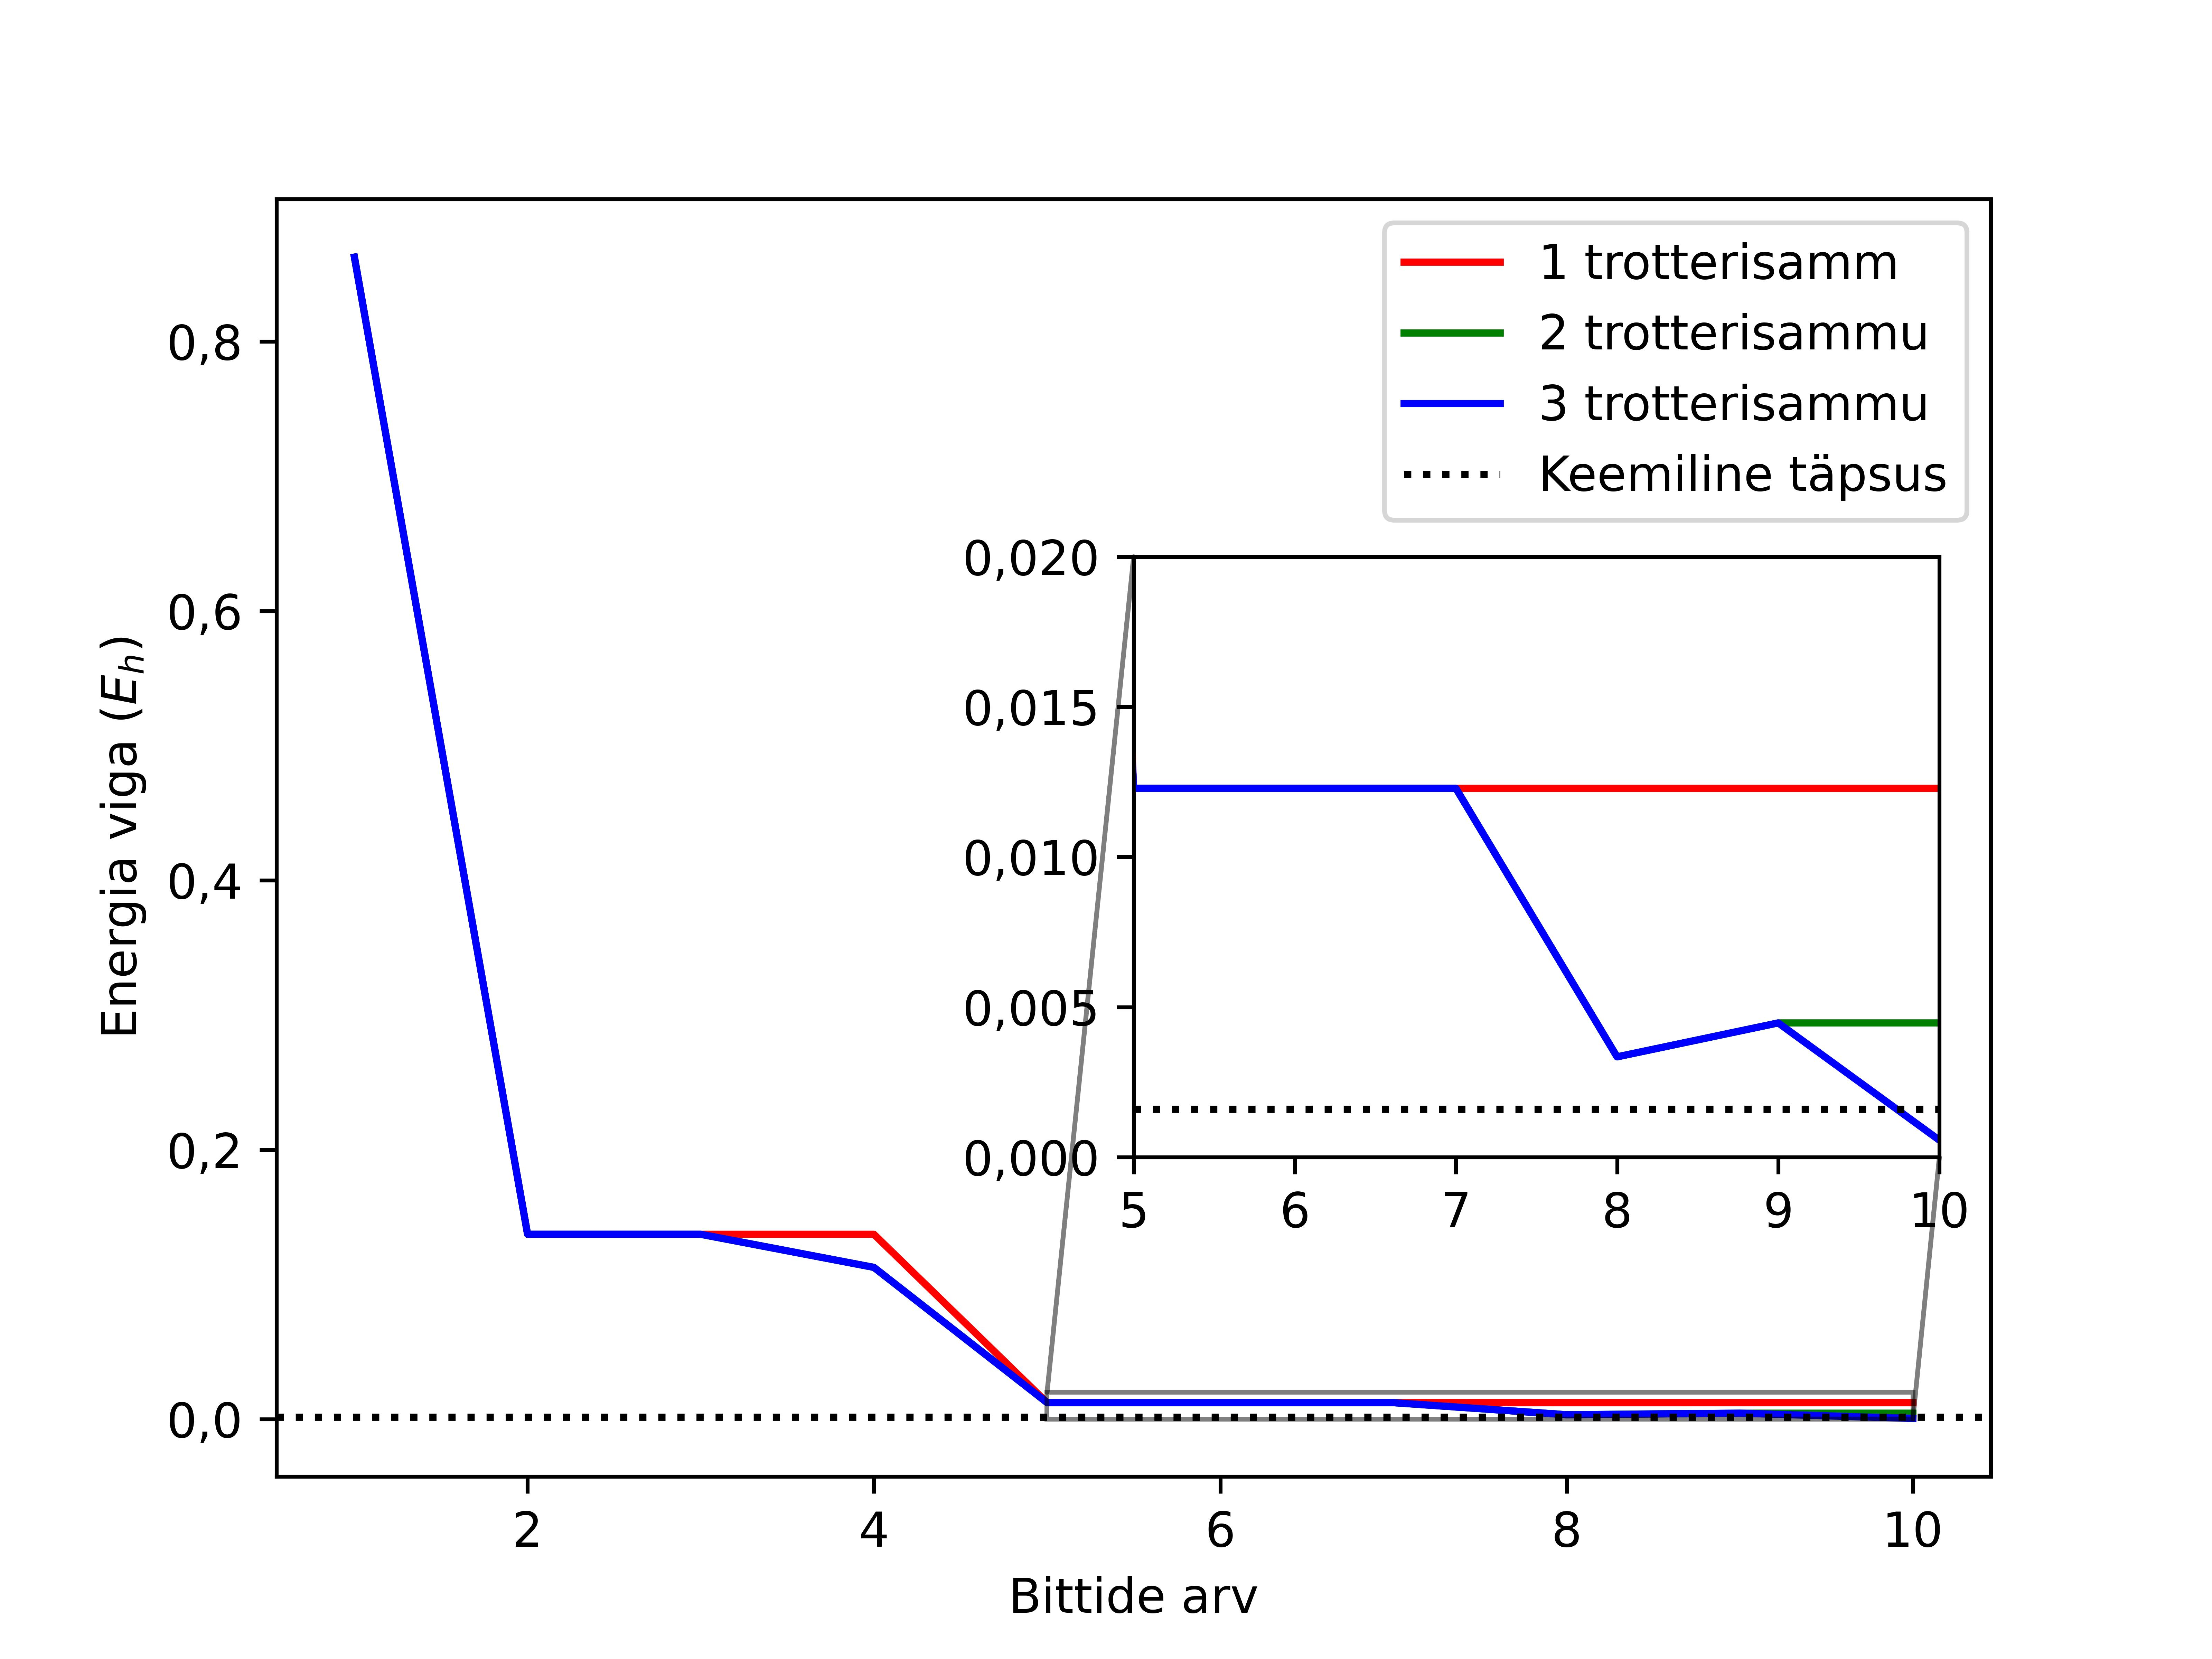
\includegraphics{trotsteps.jpg}
    \caption{Energia hinnangu sõltuvus bittide arvust. Pandagu tähele, et roheline joon on peaaegu täielilt sinese joone taga varjatud}
    \label{fig:trotsteps}
\end{figure}

Nagu näha jooniselt~\ref{fig:trotsteps} langevad ühe-, kahe- ja kolme-trotterisammused energia hinnangud hästi kokku juhul, kui energiat hinnata kahekse- või vähemakvantbitise täpsuega.
Erinevused ilmnevad alles kahekasst kvantbitist suurema täpsuse juures.
Keemiline täpsuse saavutasime kolme trotterisammu ja kümne kvantbitiga.

Parimal juhul on võimalik saavutada vaid nii suur täpsus, kui keemilise baasi valik lubab.

Trotterisammude arvu suurendamisel kasvab ahela pikkus ja seega ka kätamisaeg eksonentsiaalselt.

Kvantbittide arvust sõltub käitamisaeg kahte moodi.
Esiteks, rohkem kvantbitte tähendab pikemat käitamisaega.
Teiseks, kui faasi hindamiseks kasutada rohkem kvantbitte, siis kasvab eksponentsiaalselt ka ahela pikkus.

\begin{figure}[h]
    \centering
    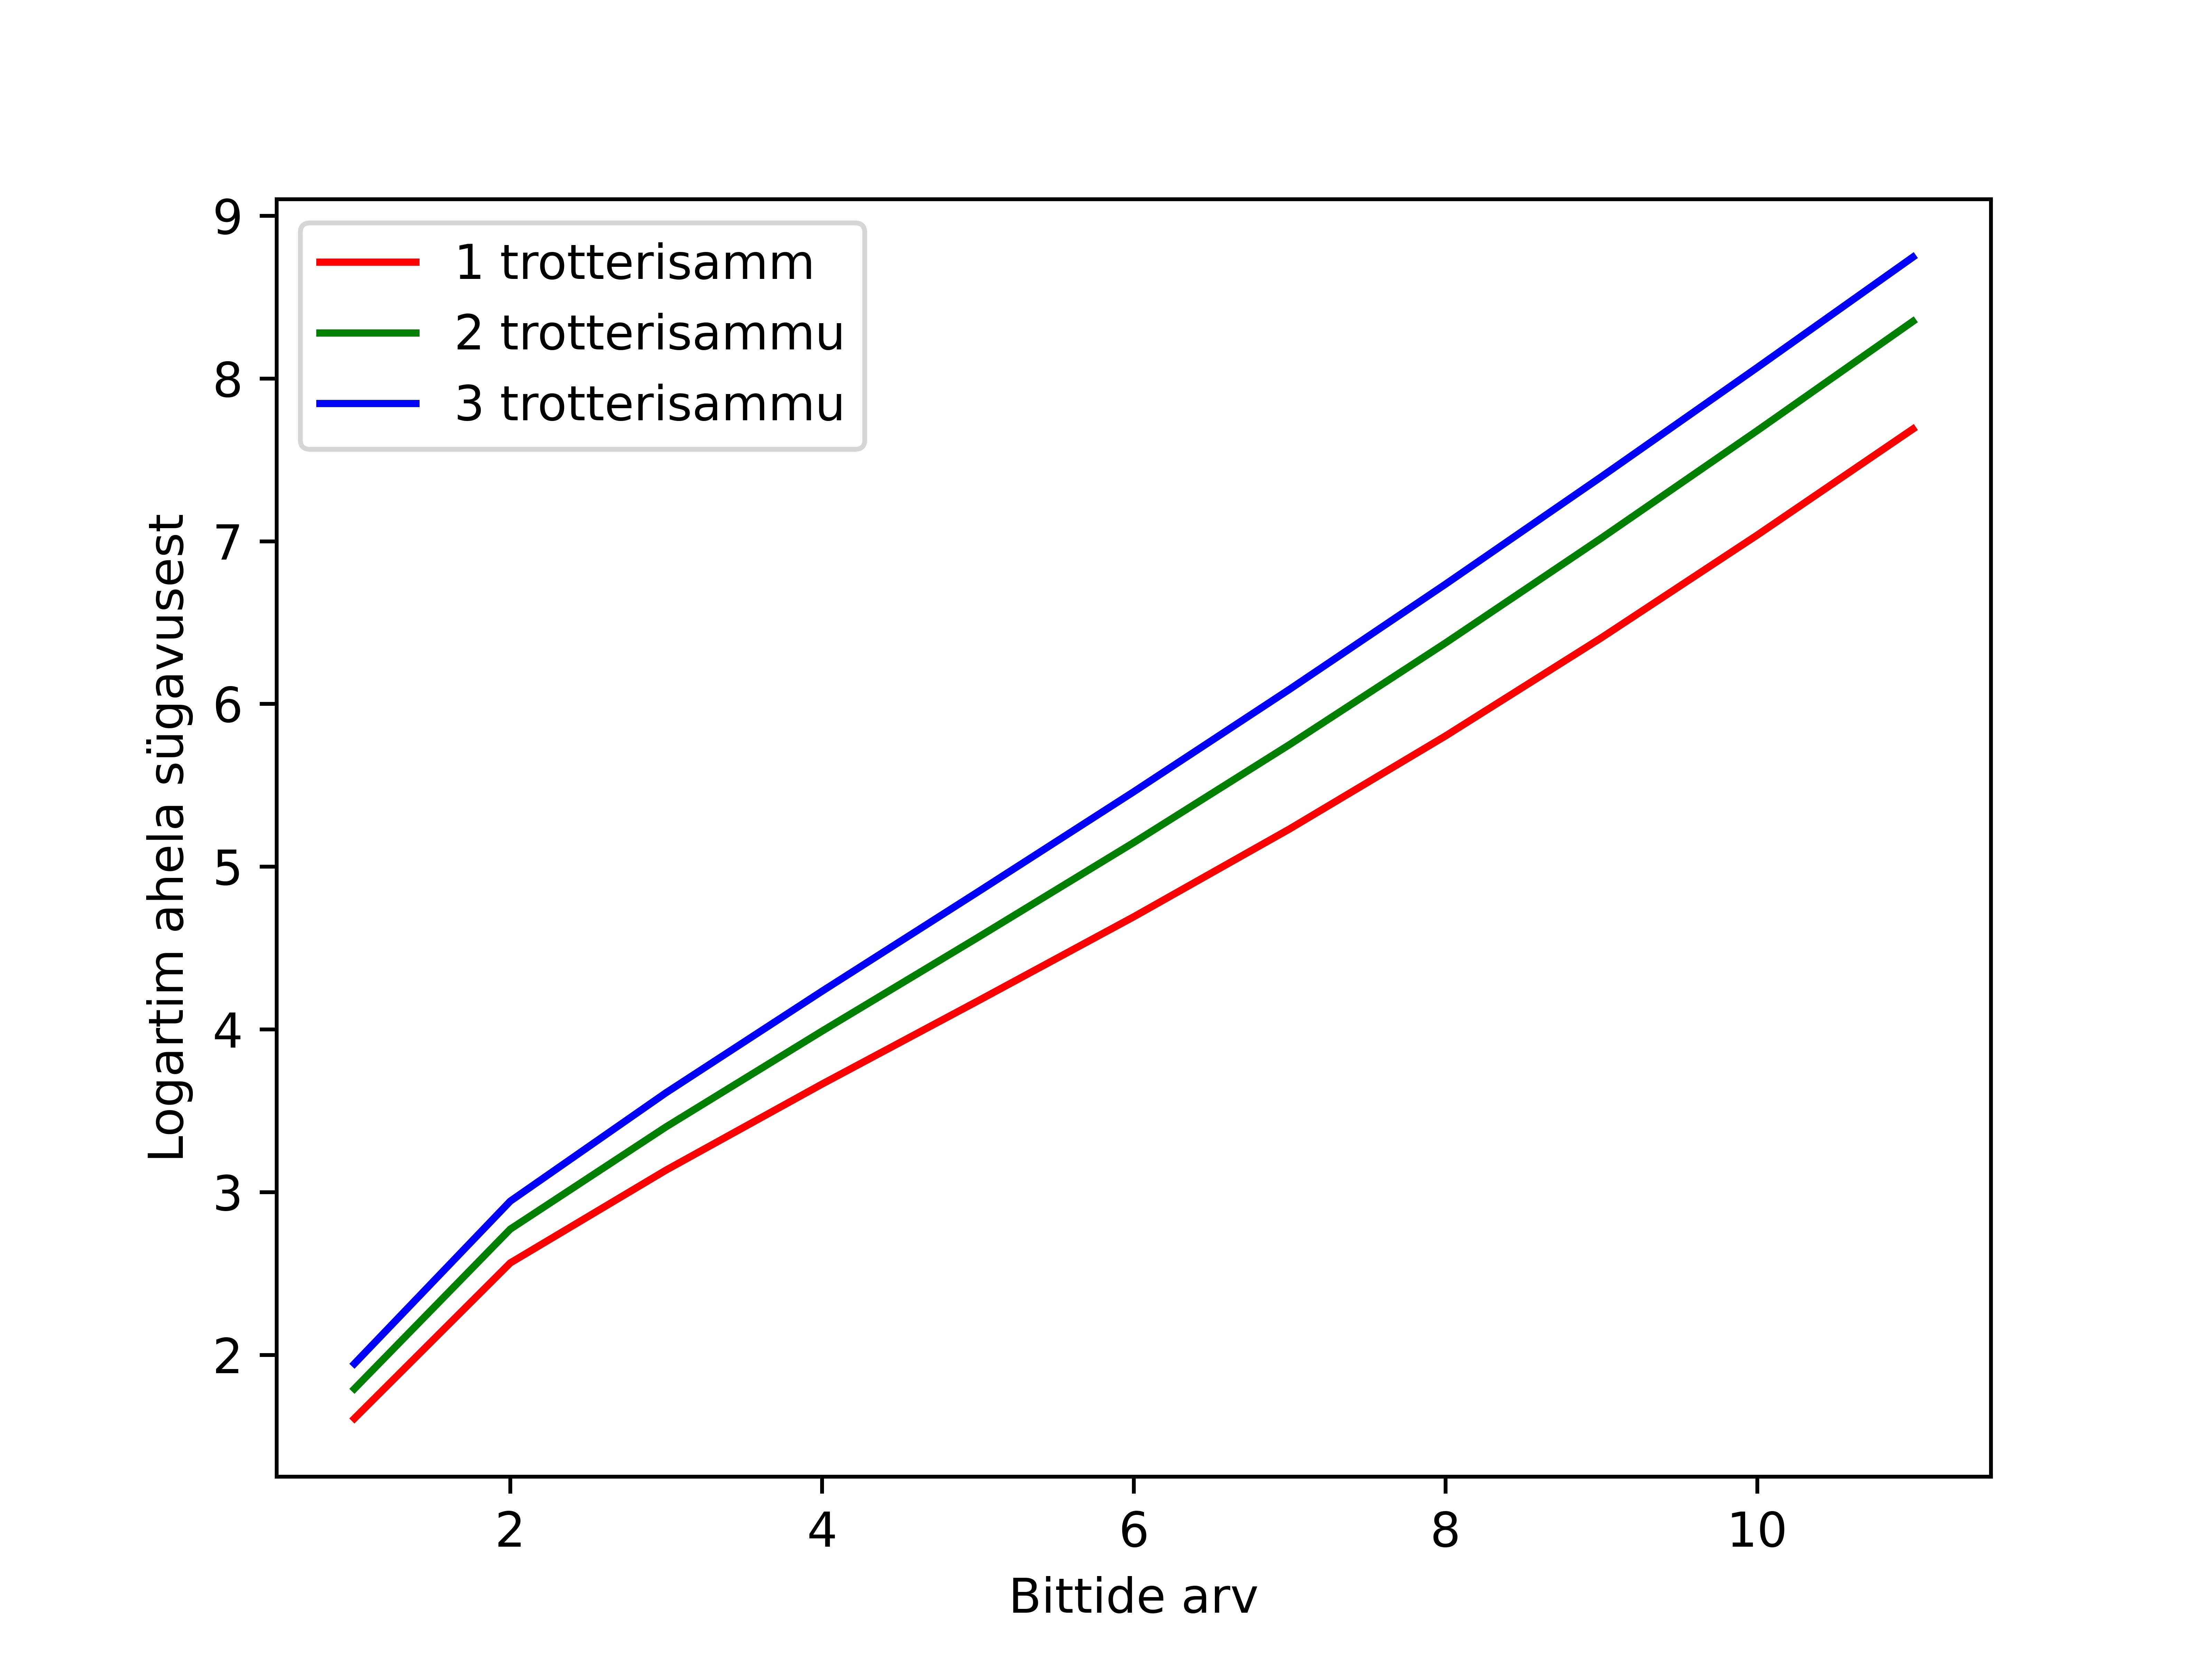
\includegraphics{depths.jpg}
    \caption{Ahela sügavuse sõltuvs bittide arvust}
    \label{fig:depths}
\end{figure}

Joonisel~\ref{fig:depths} on näidatud ahela sügavuse, st ahelas olevat kvantväravate arvu, sõltuvus kvantbittide arvust erinevat trotteri sammude arvu jaoks.
Praktiliselt on teostatav kümne kvantbiti kasutamine.


\section{Eneriga piirväärtus}

Samuti sõltub energia hinnangu täpsus energia piirväärtuse valikust, mida kujutab joonis~\ref{fig:bounds}.

\begin{figure}[h]
    \centering
    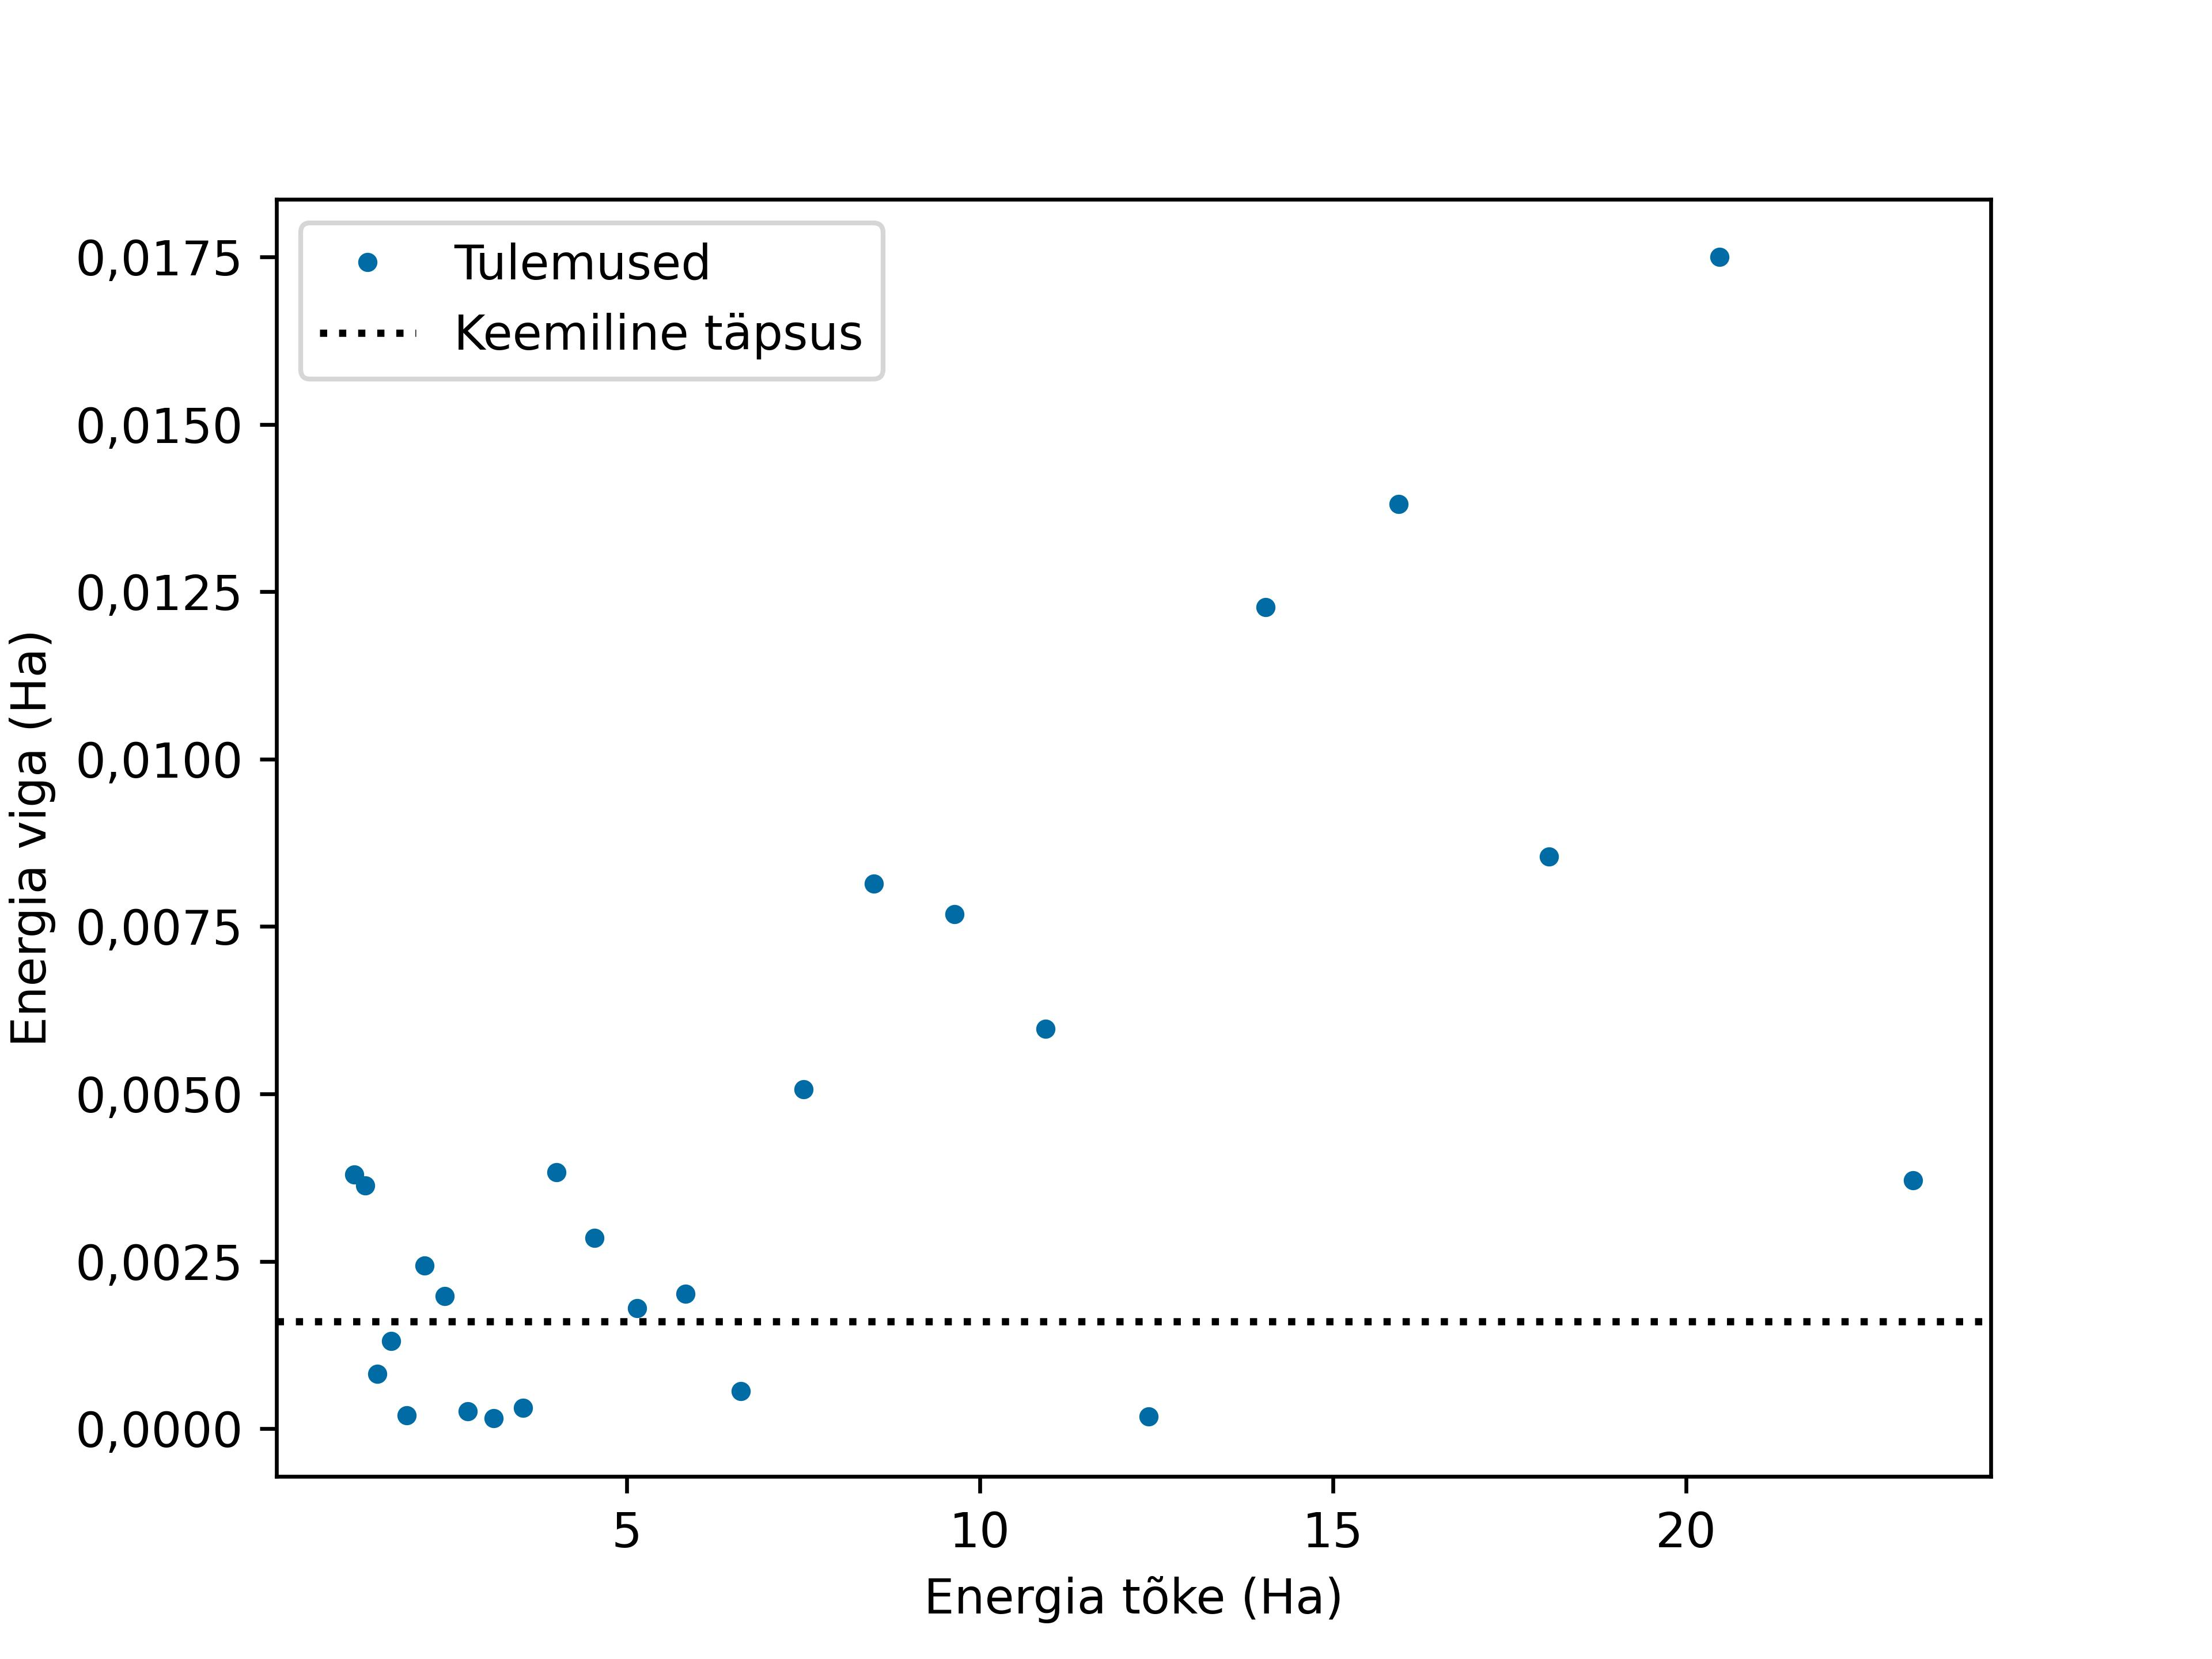
\includegraphics{bounds.jpg}
    \caption{Energia hinnagu sõltuvus energia piirväärtuse valikust}
    \label{fig:bounds}
\end{figure}

Nagu näha, sõltub energia hinnagu täpsus piirvääruse valikust kaootiliselt.
Siiski energiast oluliselt suuremate piirväärtuste puhul (mida joonisel~\ref{fig:bounds} pole kujutatud), täpsus reeglina väheneb.
Nimelt on sellisel juhul \(\phi \ll 1\) ja seega ei panusta esimesed kvantbitid tulemuse täpsusesse.


\section{Edasiarendusi}

Faasi hindamise algoritmi peamine edasiarendus on iteratiivne faasi hindamise algoritm~\cite{mcardle+etal, omalley+etal}.

Tegemist on hübriidalgoritmiga, mis kasutab klassikalist ja kvantarvutit vaheldumisi.
Kvantarvutuslikult loetakse välja üks bitt korraga, mille põhjal koostatakse klassikaliselt uus ahel järgmise biti välja lugemiseks.

Sellise algoritmi eeliseks on, et faasi hindamise registrisse on vaja vaid ühte kvantbitti.
Samuti on ahelad lühemad.

Puuduseks on keerulisus ja asjaolu, et võimalik viga mõne biti välja lugemisel võib kumuleeruda.



\chapter{Kokkuvõte}

Käesolevas töös uuriti molekulaarse süsteemi põhienergia leidmist
kvantarvutusliku faasi hindamise algoritmi abil.

\printbibliography[heading=bibintoc, title=Kirjandus]



\end{document}
